%# -*- coding: utf-8-unix -*-
%%==================================================
%% thesis.tex
%%==================================================

% 双面打印
\documentclass[master, fontset=adobe, openright, twoside, zihao=-4]{sjtuthesis}
% \documentclass[bachelor, fontset=adobe, openany, oneside, zihao=-4, submit]{sjtuthesis} 
% \documentclass[master, adobefonts, review]{sjtuthesis} 
% \documentclass[%
%   bachelor|master|doctor,	% 必选项
%   fontset=adobe|windows,  	% 只测试了adobe
%   oneside|twoside,		% 单面打印,双面打印(奇偶页交换页边距,默认)
%   openany|openright, 		% 可以在奇数或者偶数页开新章|只在奇数页开新章(默认)
%   zihao=-4|5,, 		% 正文字号:小四、五号(默认)
%   review,	 		% 盲审论文,隐去作者姓名、学号、导师姓名、致谢、发表论文和参与的项目
%   submit			% 定稿提交的论文,插入签名扫描版的原创性声明、授权声明 
% ]

% 逐个导入参考文献数据库
\addbibresource{bib/thesis.bib}
% \addbibresource{bib/chap2.bib}

\begin{document}

%% 无编号内容:中英文论文封面、授权页
%# -*- coding: utf-8-unix -*-
\title{波浪干涉效应对高速船远场波系影响的机理研究}
\author{何佳益}
\advisor{Francis Noblesse教授}
\coadvisor{万德成教授}
\defenddate{2015年12月31日}
\school{上海交通大学}
\institute{船舶海洋与建筑工程学院}
\studentnumber{1130109190}
\major{船舶与海洋工程}
\degConfIns{上海交通大学}

\englishtitle{Analysis of Interference Effects on the Farfield Waves of High-Speed Vessels}
\englishauthor{He Jiayi}
\englishadvisor{Prof. Francis Noblesse}
\englishcoadvisor{Prof. Wan Decheng}
\englishschool{Shanghai Jiao Tong University}
\englishinstitute{\textsc{Depart of XXX, School of XXX} \\
  \textsc{Shanghai Jiao Tong University} \\
  \textsc{Shanghai, P.R.China}}
\englishmajor{Naval Architecture and Ocean Engineering}
\englishdefenddate{December 31, 2015}
\englishdegConfIns{Shanghai Jiao Tong University}

\maketitle

\makeenglishtitle

\makeatletter
\ifsjtu@submit\relax
	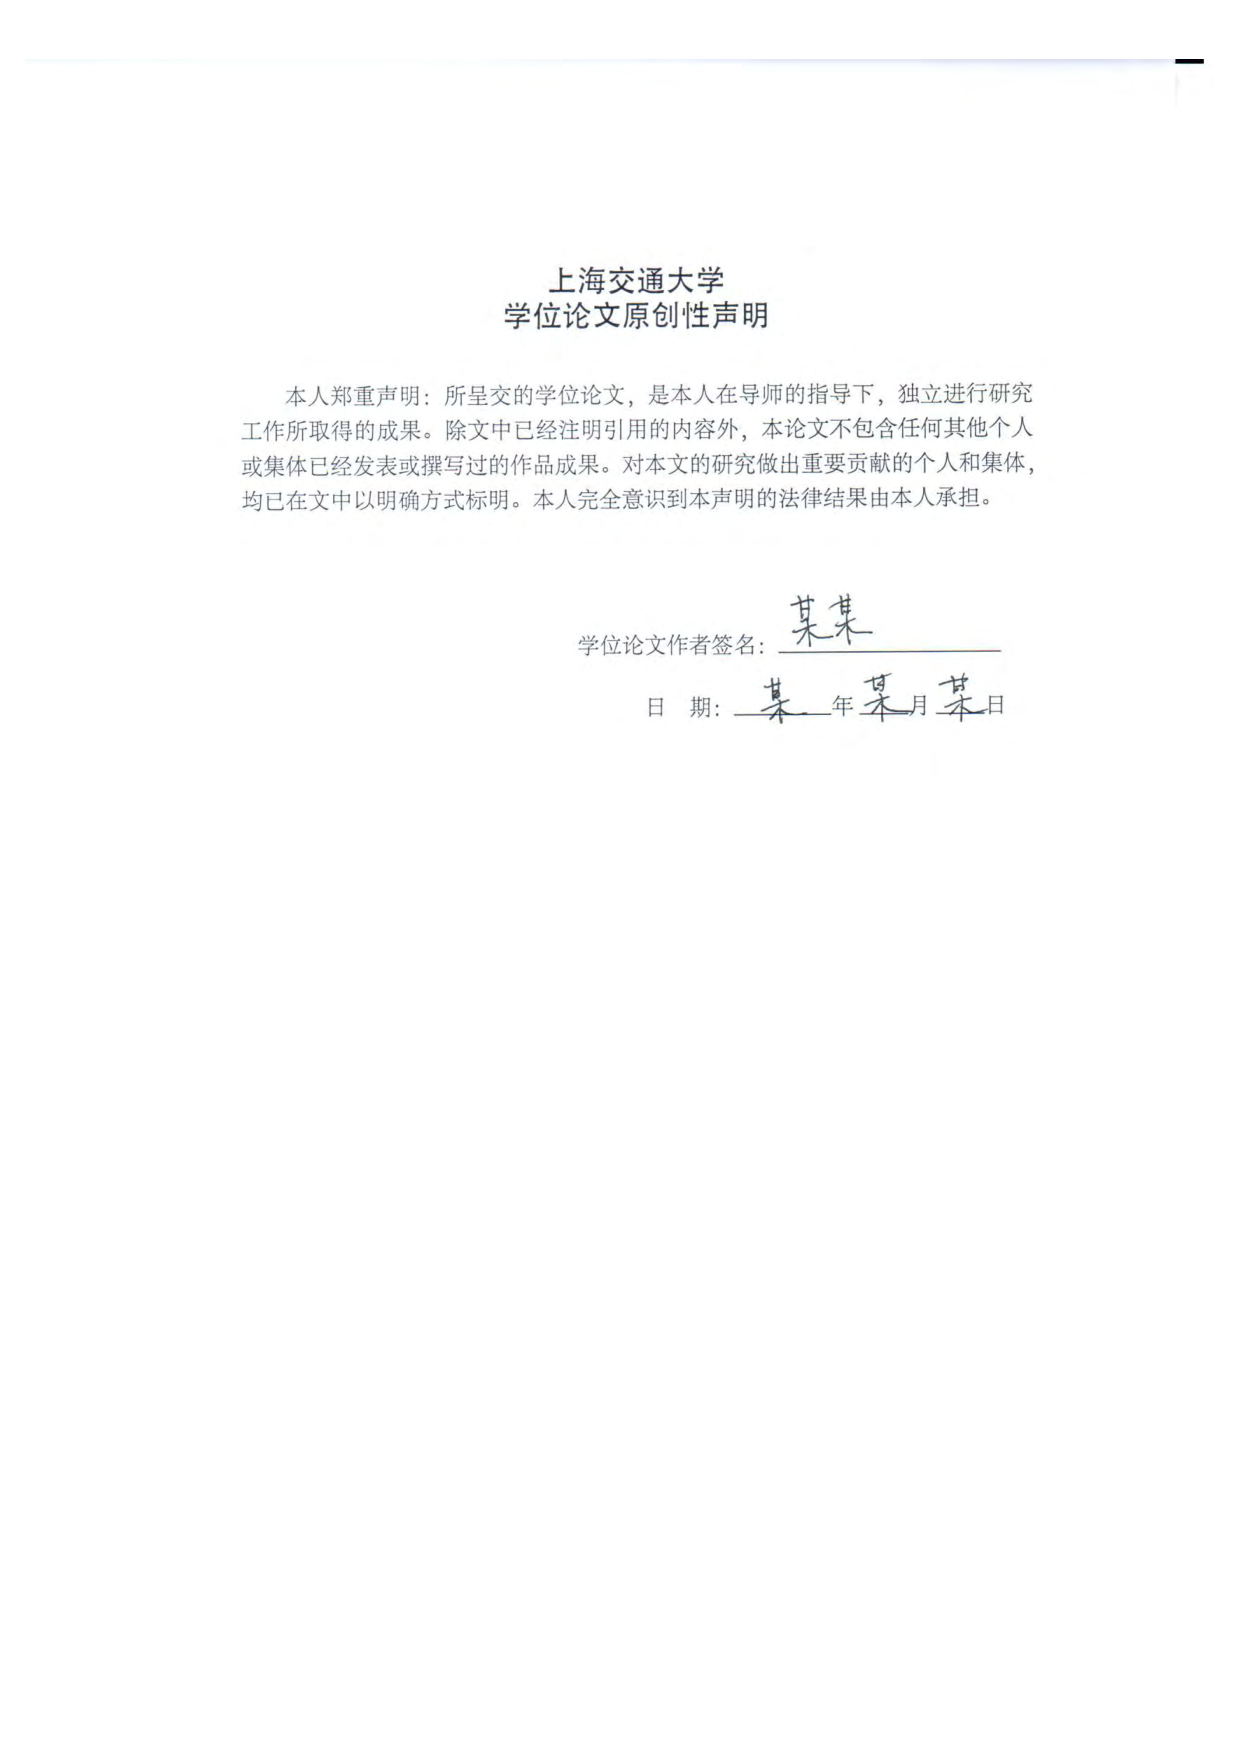
\includepdf{pdf/original.pdf}
	\cleardoublepage
	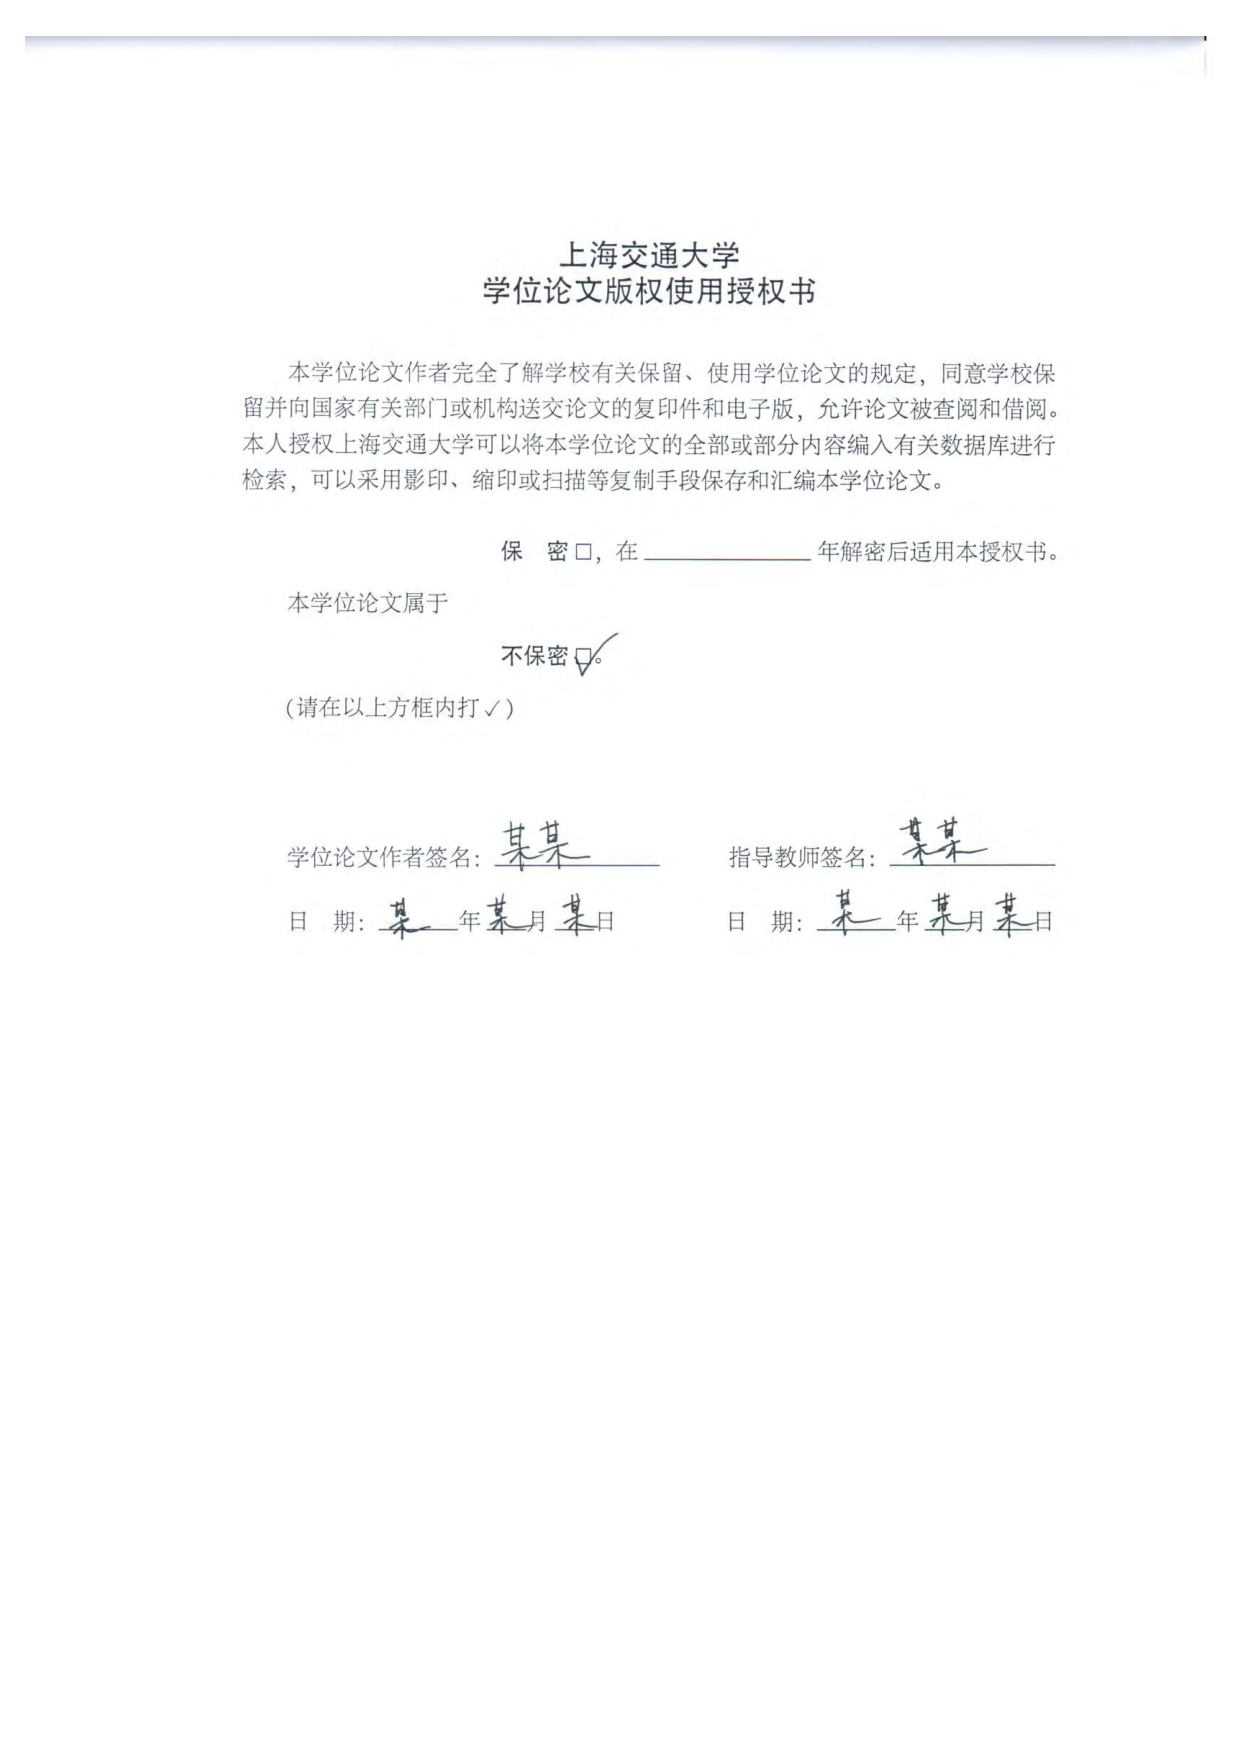
\includepdf{pdf/authorization.pdf}
	\cleardoublepage
\else
	\makeDeclareOriginal
	\makeDeclareAuthorization
\fi
\makeatother


\frontmatter 	% 使用罗马数字对前言编号

%% 摘要
\pagestyle{main}
%# -*- coding: utf-8-unix -*-
%%==================================================
%% abstract.tex for SJTU Master Thesis
%%==================================================

\begin{abstract}
很久以前人们就观察到很多船的船行波被限制在与航迹夹角
$-\psi_{\max}\le\psi\le\psi_{\max}$的锥形范围内,其中锥形半角$\psi_{\max}$
明显小于开尔文角$\psi^K\approx19^\circ28'$。很多理论已被提出以解释这些现象。
基于波浪干涉效应的两点兴波模型表明,在无限水深的静水中高速航行的单体船首尾散波间的纵向干涉或双体船
两片体首波间的横向干涉会在开尔文楔内显著小于开尔文角的射线$\psi^K$处产生波高最大的波。
本文考虑波浪干涉效应对船长$L$的单体船或船长$L$间距$S$且具有相同片体的双体船在无限水深的静水中以航速$V$航行时远场波的影响,
通过在船体表面分布的点源来代表船体。
研究报告了七艘主尺度范围广泛(长宽比、船长吃水比、型宽吃水比、半进流角)的简单船体在很大范围的弗洛德数$F\equiv V/\sqrt{gL}$
和无因次片体间距$s\equiv S/L$情况下的系统计算结果。这里,$g$为重力加速度。
单体船或双体船产生的波高最大的波所在的角度,即主要兴波角,由一种简单实用的方法获得。
这种方法基于数值确定由Hogner近似和驻相法估计的傅里叶科钦表达式中波幅函数的峰值。
本文主要的一般性结论是,尽管船行波幅值的大小受船体形状的强烈影响,但由于干涉效应造成的主要兴波角的大小受船体形状的影响很弱。
因此,与最大波高相关联的主要兴波角的大小主要是船行波的运动学特性。该发现的重要结果是,对于一般性的单体船和双体船,
主要兴波角的大小可由弗洛德数$F$和/或片体间距$s$通过简单的解析关系式得出。这些解析关系式在文中通过系统的数值计算得出。
单体船主要兴波角的解析式考虑了船首尾区域散波的纵向干涉效应和左右舷散波的横向干涉,而双体船主要兴波角的解析式还考虑了两片体产生的散波间的干涉,
因此相比两点兴波模型的初步分析给出的$\psi_{\max}$的估计更加精确。

\keywords{远场波、波浪干涉、主要兴波角、高速船}
\end{abstract}

\begin{englishabstract}
It has long been observerd that the far-field waves created by a ship that steadily
advance at high speed in calm water of large depth appear to be contained within
a wedge $-\psi_{\max}\le\psi\le\psi_{\max}$ where $\psi_{\max}$ can be significantly
smaller than the cusp angle $\psi^K\approx19^\circ28'$. Several alternative
theories have been put forward to explain this phenomenon. The two-point wavemaker
model based on wave-interference effects shows that the longitudinal interference
of waves created by the bow and the stern of a monohull ship or the lateral 
interference of waves created by the twin hulls of a catamaran can lead to largest
waves at angles that are significantly shaller that $\psi^K$. 
In this paper, the wave-interference effects on the far-field waves created by
a monohull ship of length $L$ or by a catamaran with identical twin hulls of
length $L$ at a lateral separation distance $S$, that advances at constant speed
$V$ along a straight path in calm water of large depth are considered. The hulls
are represented via a continuous distribution of sources around hull surface.
Systematic computations are performed for a wide range of Froude numbers 
$F\equiv V/\sqrt{gL}$, hull spacings $s\equiv S/L$, and seven simple 
mathematically-defined hulls that correspond to a broad range of main hull-shape
parameters (beam/length, draft/length, beam/draft, waterline entrance angle). Here,
$g$ denotes the acceleration of gravity. The dominant ray angles, where the largest
waves created by the monohull ships or the catamarans are found, are determined 
numerically via a realistic yet practical method. This method is based on the 
numerical determination of the peaks of the amplitude function in the Fourier-Kochin
representation of far-field ship waves, evaluated by means of the Hogner 
approximation, and the stationary-phase approximation. 
The main general conclusion of the study is that, although the amplitudes of 
the waves created by a ship are strongly influenced by the hull geometry 
(as well known), the dominant ray angles associated with the largest waves created 
by a ship (due to interference effects) only weakly depend on the hull geometry. 
Thus, the ray angles associated with the dominant waves are mostly a kinematic 
feature of the waves created by a ship. An important practical consequence of this 
finding is that the wake angles that correspond to the dominant waves created by a 
ship can be explicitly determined in terms of the Froude number $F$ for monohull 
ships, or in terms of the Froude number $F_s$ and the hull spacing $s$ for 
catamarans, via simple analytical relations. 
These relations, obtained via systematic numerical computations, are given here.
The numerical determined dominant ray angles take into account 
the longitudinal interference effects of the waves created by the bow and the stern
as well as the lateral interfence effects of the waves created by the port and 
starboard side of the monohull ship and by the twin hulls of the catamran. Thus,
the analytical relations obtained here provide more accurate predictions of
the dominant ray angles $\psi_{\max}$ of high-speed monohull ships and catamarans
than that derived by the simple two-point wavemaker model.

\englishkeywords{farfield waves, interference effects, dominant ray angles, 
high-speed vessels}
\end{englishabstract}



%% 目录、插图目录、表格目录
\tableofcontents
\listoffigures
\addcontentsline{toc}{chapter}{\listfigurename} %将插图目录加入全文目录
\listoftables
\addcontentsline{toc}{chapter}{\listtablename}  %将表格目录加入全文目录
% \listofalgorithms
% \addcontentsline{toc}{chapter}{代码索引}  %将表格目录加入全文目录

%%# -*- coding: utf-8-unix -*-
\chapter{主要符号对照表}
\label{chap:symb}

\begin{longtable}{rl}
$\epsilon$     & 介电常数 \\
 $\mu$ 		& 磁导率 \\
 $\epsilon$     & 介电常数 \\
 $\mu$ 		& 磁导率 \\
 $\epsilon$     & 介电常数 \\
 $\mu$ 		& 磁导率 \\
 $\epsilon$ 	& 介电常数 \\
 $\mu$ 		& 磁导率 \\
 $\epsilon$     & 介电常数 \\
 $\mu$ 		& 磁导率 \\
 $\epsilon$     & 介电常数 \\
 $\mu$ 		& 磁导率 \\
 $\epsilon$     & 介电常数 \\
 $\mu$ 		& 磁导率 \\
 $\epsilon$ 	& 介电常数 \\
 $\mu$ 		& 磁导率 \\
 $\epsilon$     & 介电常数 \\
 $\mu$ 		& 磁导率 \\
 $\epsilon$     & 介电常数 \\
 $\mu$ 		& 磁导率 \\
 $\epsilon$     & 介电常数 \\
 $\mu$ 		& 磁导率 \\
 $\epsilon$ 	& 介电常数 \\
 $\mu$ 		& 磁导率 \\
 $\epsilon$     & 介电常数 \\
 $\mu$ 		& 磁导率 \\
 $\epsilon$     & 介电常数 \\
 $\mu$ 		& 磁导率 \\
 $\epsilon$     & 介电常数 \\
 $\mu$ 		& 磁导率 \\
 $\epsilon$ 	& 介电常数 \\
 $\mu$ 		& 磁导率 \\
 $\epsilon$     & 介电常数 \\
 $\mu$ 		& 磁导率 \\
 $\epsilon$     & 介电常数 \\
 $\mu$ 		& 磁导率 \\
 $\epsilon$     & 介电常数 \\
 $\mu$ 		& 磁导率 \\
 $\epsilon$ 	& 介电常数 \\
 $\mu$ 		& 磁导率 \\
 $\epsilon$     & 介电常数 \\
 $\mu$ 		& 磁导率 \\
 $\epsilon$     & 介电常数 \\
 $\mu$ 		& 磁导率 \\
 $\epsilon$     & 介电常数 \\
 $\mu$ 		& 磁导率 \\
 $\epsilon$ 	& 介电常数 \\
 $\mu$ 		& 磁导率 \\
 $\epsilon$     & 介电常数 \\
 $\mu$ 		& 磁导率 \\
 $\epsilon$     & 介电常数 \\
 $\mu$ 		& 磁导率 \\
 $\epsilon$     & 介电常数 \\
 $\mu$ 		& 磁导率 \\
\end{longtable}
 % 主要符号、缩略词对照表

\mainmatter	% 使用阿拉伯数字对正文编号

%% 正文内容
\pagestyle{main}
%# -*- coding: utf-8-unix -*-
%%==================================================
%% chapter01.tex for SJTU Master Thesis
%%==================================================

\chapter{绪论}
\label{chap:intro}



\section{研究背景和意义}
\label{sec:background}

船舶在无限深广的静水中直线航行产生的波系最早由开尔文给出
\supercite{Thomson1887ship}。
根据开尔文的分析,船后的波系被限制在一个与航迹夹角$-\psi^K\le\psi\le\psi^K$的楔形
区域中,角$\psi^K\approx19^\circ28'$称为开尔文角。在该楔形区域内每一点都存在两种波,
即横波和散波。从开尔文的分析中还可看出,由横波和散波组成的波系其波形与船长$L$或船型
都无关,只取决于航速$V$。因此,开尔文波系与弗洛德数$F\equiv V/\sqrt{gL}$无关,
且对于任何船型---不论是单体船、双体船、潜艇,还是气垫船等---都是相同的。
具体来说,开尔文波系决定于无因次化的坐标$(X,Y)g/V^2$,其中$g$是重力加速度。
图\ref{fig:kelvinwake}显示了开尔文波系。
许多观测和数值计算结果表明,常见的排水型船舶其船行波与开尔文波系非常相似,
且波系中波高最大的波位于$\psi=\pm\psi^K$的射线上,这也和开尔文的分析一致。

\begin{figure}[htp]
  \centering
  \captionstyle{\centering}
  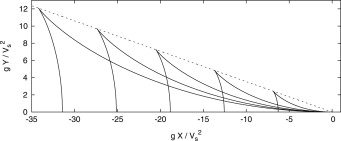
\includegraphics[width=0.5\textwidth]{chap1/kelvinwake.jpg}
  \bicaption[fig:kelvinwake]{开尔文波系}{在无限深广的静水中直线航行的船舶产生的开尔文波系,由横波和散波组成}{Fig}{The classical Kelvin pattern of 
    transverse and divergent waves created by a ship that advances at constant speed in calm water of large depth}
\end{figure}

然而大量由安装在卫星上的高分辨率合成孔径雷达(Synthetic-apeture radar, SAR)
拍摄的船行波照片显示,
船行波中最明显的波位于$\psi=\pm\psi_{\max}$的射线上,其中$\psi_{\max}$显著小于开尔文
角$\psi^K$\supercite{Taylor1910Resistance,Baker1915Ship,Munk1987Ships,Brown1989Observations,Reed2002Ship,Fang2011Kelvin,Rabaud2013Ship}。
这些窄V字形尾迹在图中呈现明亮的边缘,表明边缘的雷达后向散射 (radar backscatter) 
增强,而窄V字形内部呈现暗色,表明雷达后向散射较弱\supercite{Reed2002Ship}。
这里将$\psi_{\max}$称为主要兴波角(dominant wake angle)。
特别地,\parencite{Rabaud2013Ship}报告了37例不同船舶在不同航速下的主要兴波角
$\psi_{\max}$数据,其弗洛德数$F$分布于$0.1<F<1.7$。其中处于$0.6<F$的12个观测数据显示
,主要兴波角$\psi_{\max}$一致并显著地小于开尔文角$\psi^K$,且主要兴波角$\psi_{\max}$
随弗洛德数$F$的增大而减小。而处于$0.1<F<0.6$区域的主要兴波角$\psi_{\max}$大致位于开
尔文角$\psi^K$附近。
图\ref{fig:rabaudobserv}显示了\parencite{Rabaud2013Ship}的观测结果。

\begin{figure}[htp]
  \centering
  \captionstyle{\centering}
  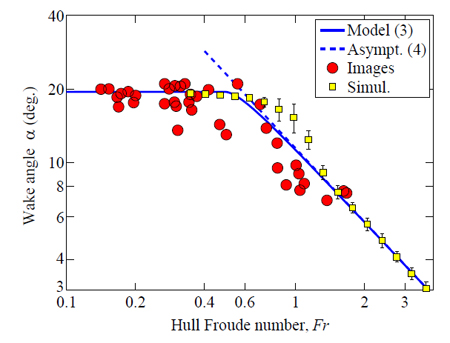
\includegraphics[width=0.5\textwidth]{chap1/expRM.jpg}
  \bicaption[fig:rabaudobserv]{观测的主要兴波角$\psi_{\max}$与弗洛德数$F$的关系}
  {由\parencite{Rabaud2013Ship}观测的37艘船的主要兴波角$\psi_{\max}$与弗洛德数$F$
的关系}{Fig}{Relation between the dominant wake angles $\psi_{\max}$ and the Froude 
numbers $F$ of 37 observed narrow V-shaped ship wakes}
\end{figure}

众所周知,开尔文的经典分析\supercite{Thomson1887ship}是水波理论的基础,几乎出现在
任何一本介绍水波和水动力学的书籍中,如
\parencite{newman1977marine,sheng2003principle}。
而观测到主要兴波角$\psi_{\max}$显著小于开尔文角$\psi_{\max}$的现象表面上与开尔文的
理论相悖。因此解释这一现象十分具有重要的理论意义。

船体阻力按产生阻力的原因来分类,则船体总阻力$R_t$由兴波阻力$R_w$、摩擦阻力$R_f$和
粘压阻力$R_{pv}$三者组成:$R_t=R_w+R_f+R_{pv}$。
船行波是产生兴波阻力的原因\supercite{Michell1898wave,Wehausen1973Wave},
而兴波阻力是船舶阻力的重要组成部分,特别是对高速船,兴波阻力占总阻力的40\%-50\%。
根据弗洛德定律,对于给定船型,船体兴波阻力系数$C_w$仅仅是弗洛德数$F$的函数。
对于较丰满船,兴波阻力系数$c_w$随弗洛德数$F$的增加快速增加,而当$F\approx0.4$时,
船首波的波长约等于船长$\Lambda\approx L$,此时船就像深陷在首波波峰后的槽中一样,因此
兴波阻力系数急剧增加。与该弗洛德数对应的航速称为船身极速 (hull speed)。
滑行 (planing) 是克服船身极速的方式之一,但是很多现代排水型船无需滑行即可轻易克服
船身极速。随着$F$的增大,$C_w$继续增大,瘦削船在$F=0.5$附近存在$C_w$峰值区,
当$F>0.5$时,$C_w$随$F$的增大而减小。窄V字形尾迹的夹角---即主要兴波角$\psi_{\max}$
---随弗洛德数$F$减小的现象与兴波阻力系数$C_w$随弗洛德数$F$的增大而减小的现象
之间的相似性暗示窄V字形尾迹与兴波阻力之间存在联系\supercite{Rabaud2014narrow}。
\parencite{Rabaud2014narrow}还注意到
$\psi_{\max}$随$F$的增大而减小的临界弗洛德数与$C_w$开始减小的临界弗洛德数的数值
相差不大。因此研究这一问题也有助于增加对兴波阻力的认识,从而为减小船舶阻力、
提高船舶快速性提供新的视角。

SAR图像中经常出现船舶尾迹,通过分析这些尾迹可以获得关于船舶的信息。
因此SAR图像是得到实用的船舶数据的重要来源。
由此获得的数据可以与基于船舶自我报告的船舶自动识别系统
(Automatic Identification System, AIS) 中的数据进行对比验证。
除了用来验证AIS系统中的数据,这些信息还可能被用来对海域进行广域监视
(wide area surveillance)。现代SAR传感器在短时间内就能产生大量数据,
这对自动舰船尾迹检测 (automatic ship wake detection) 产生了需求
\supercite{Crisp2004state}。
对窄V字形尾迹的理解关乎能否从SAR图像中得到关于船舶的有用信息
\supercite{Tunaley2009narrow}。

\section{国内外发展现状}
\label{sec:statofart}

\subsection{窄V字形船行波的理论分析}
针对主要兴波角$\psi_{\max}$显著小于开尔文角$\psi^K$的现象,许多研究者给出了解释。
\parencite{Brown1989Observations}将主要兴波角$\psi_{\max}$处的波与非线性孤立波的特征
进行了对比,并认为主要兴波角$\psi_{\max}$的产生可能是因为该处非线性孤立波的存在。
\parencite{Mei1991Note}认为由周围环境的波浪造成的船舶运动可能是产生该非线性孤立波的
原因。\parencite{Zhu2008Resonant}的研究显示了船行波与环境波浪的三阶共振干涉会在
开尔文波系内产生新的波。此波所处的角度与船舶航速和波浪参数有关。
而\parencite{Shugan2006Kelvin}的研究表明,环境波浪的存在本身就会改变开尔文波系
的楔形夹角。如果船舶航向与波浪传播方向一致,楔形区域的夹角将会变小。
\parencite{Fang2011Kelvin}考虑了风和有限水深对开尔文波系的影响。
在水深弗洛德数$F_h>1$时,开尔文角随$F_h$的增大而减小。
虽然开尔文的分析中未考虑到的因素---非线性、船舶摇荡运动、环境波浪、风、有限水深---
会显著地影响开尔文波系,这并不表示观测的主要兴波角$\psi_{\max}$
小于开尔文角的现象是由于这些因素引起的。

\parencite{Rabaud2013Ship}在线性水波理论的基础上,引入了下列假设:
船舶兴波的波长不能超过船长。因此,一旦兴波的波速达到与波长等于船长对应的波速后
便无法增加。他们的分析表明,当弗洛德数$F>0.5$时主要兴波角$\psi_{\max}$
的大小与$F$成反比。\parencite{Moisy2014Mach}与\parencite{Moisy2014Scaling}
又将上述假设应用到非轴对称形的自由面压力分布的兴波与考虑表面张力的情况下,
也得到类似结论。虽然\parencite{Rabaud2013Ship}得出的解析关系$\psi_{\max}(F)$
与该文中的观测结果相对一致,然而文中并未就其引入的假设提供任何解释。
众所周知,在线性水波理论的框架下,开尔文波系中波长最大的波传播方向为船舶的航向,
其(无因次)波长为$\lambda^{\max}\equiv\Lambda^{\max}/L=2\pi F^2$,
因此当弗洛德数$F>0.4$时,波长大于船长。
可见\parencite{Rabaud2013Ship}中的假设是违背线性水波理论的。
因此如果没有其他证据支持该假设,很难使人信服。事实上,\parencite{He2015Comparison}
论证了在线性水波理论的框架下,波长不超过某截断波长$\lambda<\lambda^{cut}=1$的假设
在数学上与兴波角度不超过某截断兴波角$\psi<\psi^{cut}$是完全等价的。具体来说,
\begin{equation}
  \lambda\le\lambda^{cut}
  \label{eq:rabaudassump}
\end{equation}
等价于
\begin{equation}
  \psi\le\psi^{cut}\equiv\tan^{-1}\left(
  \frac{\sqrt{\lambda^{\max}/\lambda^{cut}-1}}{2\lambda^{\max}/\lambda^{cut}-1}
  \right)
  \label{eq:wavlencut}
\end{equation}
所以限制了波长不能超过船长,自然也就限制了兴波角不能超过某个角度。
因此,\parencite{Rabaud2013Ship}的解释存在逻辑错误。

\parencite{Darmon2014Kelvin}考虑了高斯分布的压力场的自由面兴波,从理论分析中证明了
波幅最大的波所处的射线其角度按$F^{-1}$的形式减小。\parencite{Darmon2014Kelvin}的结果
暗示SAR观测到的主要兴波角$\psi_{\max}$很可能就是波幅最大的波所处的射线的角度。
相比其他解释,其优美之处在于首次从波幅的大小解释窄V字形船行波的出现\supercite{Dias2014Ship}。
\parencite{Darmon2014Kelvin}的结果也表明了即使不考虑非线性、船舶摇荡运动、环境波浪、
风、有限水深等这些外部因素,只用线性势流理论也能产生窄V字形船行波。
\parencite{Benzaquen2014Wake}将\parencite{Darmon2014Kelvin}的结果推广到各向异性
的自由面压力分布形式,并得到相似结论。在\parencite{Darmon2014Kelvin}对主要兴波角
$\psi_{\max}$理解的基础上,\parencite{Pethiyagoda2014What}和\parencite{Pethiyagoda2015Wake}
研究了非线性和有限水深效应对主要兴波角$\psi_{\max}$的影响,\parencite{Ellingsen2014Ship}
研究了剪切流对主要兴波角$\psi_{\max}$的影响。当弗洛德数$F\gg1$时,主要兴波角
$\psi_{\max}$随弗洛德数$F$的变化规律几乎不受剪切流的影响。
虽然\parencite{Darmon2014Kelvin}展示了主要兴波角也即波幅最大的波所对应的角
$\psi_{\max}$随弗洛德数$F$的增大而减小的关系,但其并未解释出现这种现象的原因。


需要指出的是,不同的船舶在船长、航速、船型上有很大差别,它们产生的船行波也大不相同。
比如说,全部浸入水中的潜艇或低速排水型船(如油轮)产生的波系主要包括横波,
而高速艇产生的波系中散波占主导。事实上,船行波的波形很大程度上受弗洛德数$F$和
船体表面形状的影响。这并不与开尔文的结论矛盾。开尔文基于驻相点法
(method of stationary phase) 的渐近分析只考虑波的相位,没有也不能考虑横波和散波的
波幅。而横波和散波的波幅在被开尔文角包括的船后楔形区域内变化,
且很大程度上受弗洛德数$F$和船体表面形状的影响。这是产生多种多样的船行波的原因。

回顾开尔文的压力点兴波理论,开尔文波系实际上是开尔文根据流体力学理论求得的一个压力点
在水面上作匀速直线运动时的波形图。而船行波正是由于船舶在水面上航行时船体周围流体压力
变化引起的。最大压力区产生于船体首尾驻点附近,其兴波作用最强,因此这两个最大压力区的
兴波可以简化为两个压力点兴波的叠加。考虑两个压力点的兴波也意味着引入了新的物理量:
长度。因此考虑船舶首尾波系之间的干涉成为可能。事实上,船舶工程师通常利用首尾横波的
干涉选择船长,力求避免波阻峰点,设法处于波阻谷点\supercite{sheng2003principle}。
然而首尾散波的干涉并未引起人们的重视。

\parencite{Noblesse2014Why}首先从波浪干涉的角度解释窄V字形船行波的出现。
\parencite{Noblesse2014Why}证明了主要兴波角$\psi_{\max}$处波幅最大是由高航速时
散波的相长干涉效应 (constructive interference) 造成的。众所周知,在线性势流理论的
框架下,船体的兴波速度势可以表示成在船体表面上分布的点源兴波速度势的叠加\supercite{Noblesse2011Practical,Noblesse2013Neumann}。
\parencite{Noblesse2014Why}将单体船简化为位于首尾的两个兴波点,将双体船简化为位于两
片体首部的两个兴波点,从而引入长度参数:船长$L$与片体间距$S$。图展示了产生于单体船
首部和尾部区域的两开尔文波系的线性叠加。类似地,图展示了产生于双体船两片体首部区域
的两开尔文波系的线性叠加。

\begin{figure}[htp]
  \centering
  \captionstyle{\centering}
  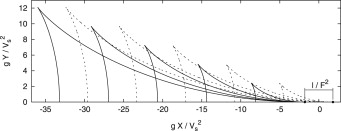
\includegraphics[width=0.5\textwidth]{chap1/longKel.jpg}
  \bicaption[fig:longintrf]{单体船首尾波系的叠加}
  {位于单体船首尾区域的两兴波点产生的开尔文波系的叠加}{Fig}
  {Superposition of two Kelvin wave patterns with origins (marked as dots)
located at the bow and the stern of a monohull ship}
\end{figure}

\begin{figure}[htp]
  \centering
  \captionstyle{\centering}
  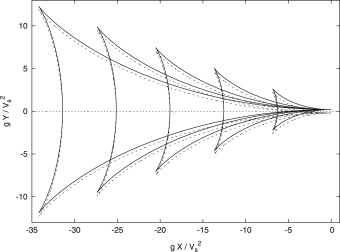
\includegraphics[width=0.5\textwidth]{chap1/latKel.jpg}
  \bicaption[fig:longintrf]{双体船两片体首波系的叠加}
  {位于双体船两片体首部的两兴波点产生的开尔文波系的叠加}{Fig}
  {Superposition of two Kelvin wave patterns with origins (marked as dots)
located at the bows of the twin hulls of a catamaran}
\end{figure}

定义如下弗洛德数
\begin{subequations}\label{eq:Fdef}
  \begin{eqnarray}
    F\equiv V/\sqrt{gL} \label{eq:Fdef-a}\\
    F_s\equiv V/\sqrt{gS}
    \label{eq:Fdef-b}
  \end{eqnarray}
\end{subequations}
\parencite{Noblesse2014Why}证明当$F>F^x$时,单体船首尾兴波的散波成分间的纵向干涉
(longitudinal interference) 会在与航迹成$\psi=\pm\psi^x_{\max}$的射线上产生波高最大
的波。$F^x$与$\psi^x_{\max}$由下式给出
\begin{subequations}\label{eq:psixym}
  \begin{equation}
    \psi^x_{max}\approx\arctan(0.16\ell_e/F^2),\quad F^x\approx 0.59
    \label{eq:psixm}
  \end{equation}
这里,$\ell_e$是位于船首的点源与位于船尾的点汇之间的距离。考虑到首波的波峰总是
出现在船首偏后位置,而尾波的波谷出现船尾靠前位置,工程上常用$\ell_e\approx0.9$
表示这段距离。

类似地,当$F_s>F_s^y$时,双体船两片体首部兴波的散波成分间的横向干涉 
(lateral interference) 会在与航迹成$\psi^y_{\max}$的射线上产生波高最大的波。
$F^y_s$与$\psi^y_{\max}$由下式给出
\begin{equation}
  \psi^y_{\max}\approx\arctan(0.2/F_s),\quad F^y_s\approx 0.37
  \label{eq:psiym}
\end{equation}
\end{subequations}

式\eqref{eq:psixm}与\eqref{eq:psiym}表明,由纵向干涉产生的主要兴波角$\psi^x_{\max}$
以$1/F^2$的形式减小,而由横向干涉产生的主要兴波角$\psi_{\max}^y$则以$1/F_s$的形式
减小。\parencite{Noblesse2014Why}考虑的两点兴波模型 (2-point wavemaker model) 
中的纵向干涉和横向干涉是分布在船体表面的点源间相互干涉的两种基本情况。
两点兴波模型明确揭示了主要兴波角$\psi_{\max}$小于开尔文角$\psi^K$的现象是由于波浪的
相互干涉产生的。其结果为船体兴波的主要兴波角$\psi_{\max}$提供了简单实用的估计,如图 5所示。


\begin{figure}[htp]
  \centering
  \captionstyle{\centering}
  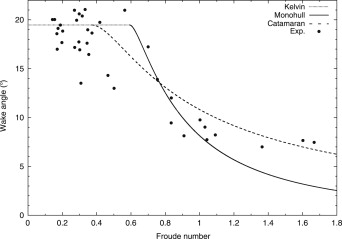
\includegraphics[width=0.5\textwidth]{chap1/longlat.jpg}
  \bicaption[fig:twopwavmkr]{两点兴波模型得出的主要兴波角$\psi_{\max}$的大小}
  {考虑单体船首尾波系以及双体船两片体首波系干涉效应的两点兴波模型预测的
    主要兴波角$\psi_{\max}$的大小}{Fig}
    {Theoretical predictions given by the two-point wavemaker model 
      of interference between the divergent waves created by the bow 
      and the stern of a monohull or between the bows of the twin 
    hulls of a catamaran}
\end{figure}

至此我们可以看到,窄V字形船行波是由高速时散波的干涉效应产生的。
两兴波点的横向或纵向相干干涉会使$\psi=\pm\psi_{\max}$射线上的波浪波高增加,
因此该处的波在观测时更容易受到注意。两点兴波模型作为开尔文压力点兴波理论的扩展,
预测的单体船和双体船的主要兴波角与观测结果基本一致,表明了该理论的正确性。
同时,我们也可以看到散波干涉对波形的影响只在高速时(对单体船而言,$F>0.59$)才明显,而一般的排水型船舶很难达到这一航速,这可能是散波干涉长期被忽视的原因之一。

虽然波浪干涉效应在以往的研究中\supercite{Mei1991Note,Zhu2008Resonant,Fang2011Kelvin,Rabaud2013Ship,Darmon2014Kelvin}
被忽视,它存在于各种各样的波动中,如光、无线电、声波、水波、物质波。
事实上,船周围流场速度由幅值随距离$h\equiv\sqrt{x^2+y^2}$以$1/\sqrt{h}$衰减的
波动部分(wave component)和以$1/(x^2+y^2+z^2)^{3/2}$衰减的局部流动部分
(local flow component)组成。在距离船相对较小的距离外,
船产生的流动主要由向外自由传播的波浪线性叠加而成。
因此波浪之间的干涉作用是决定船行波波形的最主要的物理机理。

由于两点兴波模型\supercite{Noblesse2014Why}将船体简化成两个兴波点,
模型预测的主要兴波角$\psi_{\max}$不可能非常精确。
而\parencite{Darmon2014Kelvin}虽然通过理论证明和数值计算给出了主要兴波角的解析式,
但结果基于压力的高斯分布形式。正如前面提到的,船体表面的压力分布一般在首尾驻点附近
存在最大压力区,因此这种压力分布的兴波很难代表船体的兴波(除非对于滑行艇)。
此外,\parencite{Darmon2014Kelvin}的解析式是在高弗洛德数 ($F>2$) 情况下得出的
渐近结果,即使高速船也很难达到,因此工程实用性不强。

\subsection{波形的数值计算}
考虑在线性势流理论的框架下,船长为$L$的船以航速$V$在无限深广静水中直线航行时所产生
的远场波。观察流动的参考系是固结在船体上与船体一起运动的伽利略参考系$\mathbf{X}=(X,Y,Z)$,
因而流动从参考系观察是定常的。流场的速度可以看作均匀来流的速度$(-V,0,0)$与扰动速度
$(\Phi_X,\Phi_Y,\Phi_Z)$的叠加,其中$\Phi(\mathbf{X})$是扰动速度势。将未扰动的自由
面定义为$Z=0$且$Z$轴竖直向上,$X$轴与船的航向一致且指向船首。用船长$L$以及航速
$V$定义无因次化的坐标系$\mathbf{x}\equiv\mathbf{X}/L$、扰动速度势$\phi=\Phi/VL$、
以及速度场$\nabla_\mathbf{x}\phi\equiv(\phi_x,\phi_y,\phi_z)\equiv(\Phi_X,\Phi_Y,\Phi_Z)/V$。

在线性势流理论的框架内,船体周围的流场可以表示成分布于船体表面的奇点(点源与点汇)
诱导的流场。这些奇点与满足线性自由面条件的基本解(格林函数)相联系。这些被称为自由面
格林函数的基本解已经被广泛研究\supercite{Noblesse1981Alternative}。
分布于船体表面的点源其密度可以由船体曲面形状显式表出,如Hogner近似\supercite{Hogner1932Hydromech}或者与之类似的细长船体理论\supercite{Noblesse1983slender}
(slender-ship approximation),也可通过Neumann-Kelvin (NK) 理论\supercite{Brard1972representation,Gueval1974distribution}
或与之相关的Neumann-Michell (NM) 理论\supercite{Noblesse2013Neumann}
通过数值计算确定。Hogner近似或细长船体理论分别是NM理论或NK理论的近似解
\supercite{Noblesse1983slender,Noblesse2013Neumann}。
细长船体理论与薄船理论\supercite{Michell1898wave}(thin ship theory)密切相关,
可以看作是薄船理论的延伸。

Hogner近似虽然没有NM理论精确,但是既简单又实用。特别地,基于Hogner近似预报的多艘船
在范围广泛的弗洛德数$F$区间内的升沉、纵摇、阻力和自由面升高与实验结果以及NM理论的
预报结果一致\supercite{Noblesse2013Neumann,Huang2013Numerical}。
Hogner近似将船体周围的流场显式表达成弗洛德数$F$和船体曲面形状的函数,
因而比NM理论简单得多。
在Hogner理论中,分布于船体表面的点源密度等于曲面法向量$\mathbf{n}\equiv(n^x,n^y,n^z)$的$x$分量$n^x$。


尽管薄船理论\supercite{Michell1898wave}早在1898年就被提出并被用于估算兴波阻力,
波形的计算直到一个世纪后才出现。理论上薄船理论可直接用于波形的数值模拟,
但由于每个场点的波高都需要计算一个三重积分,所以在计算机产生之前波形的模拟未能实现。
事实上,由于没有Michell积分的计算程序,薄船理论在船舶工程和水动力学实验室并未受到
大量应用。随着计算机科学的进步,现在科学家已经能够通过数值模拟获得复杂的船行波图像。
Ernie Tuck对波形计算做过深入研究。他基于薄船理论编写了快速计算波形的程序,
对于一艘驱逐舰的计算结果与试验波形吻合良好,且并不比考虑
非线性和粘性效应的程序差\supercite{Tuck1971ship,Tuck2001Ship}。
图\ref{fig:tuckwavpat}是基于薄船理论预报的一艘驱逐舰在30节航速下的波形。
值得一提的是,Tuck很早就注意到利用多体船片体之间的波浪干涉可合理布置片体位置
减小兴波阻力,并对纵向错开和不错开的双体、三体和四体船的片体位置的最有布置进行了
研究\supercite{Tuck1998Optimum}。

\begin{figure}[htp]
  \centering
  \captionstyle{\centering}
  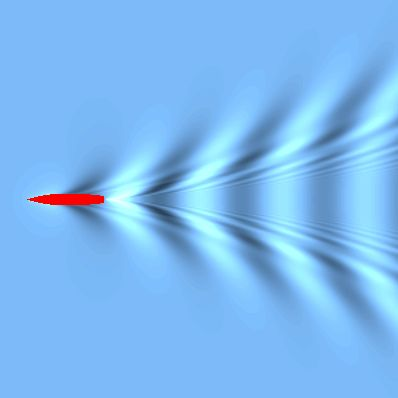
\includegraphics[width=0.5\textwidth]{chap1/eot.jpg}
  \bicaption[fig:tuckwavpat]{薄船理论预报的波形}
  {薄船理论预报的一艘驱逐舰在30节航速时的波形\supercite{Tuck2001Ship}}{Fig}
    {Wave pattern of a destroyer hull at 30 knots predicted via thin-ship theory}
\end{figure}

在线性势流理论的框架里,船行波可表示成一系列正弦波$E=e^{\mathbf{i}h\varphi}$
的线性叠加,这些波的无因次波长在$0\le\lambda\le2\pi F^2$范围内。
因此,线性势流理论得出的船行波中包含了波长非常短的短波,而这些短波在现实中由于受到
表面张力和粘性的影响不可能存在。通过线性外插法,\parencite{Noblesse2013Evaluation}
过滤掉了短波。数值计算结果与试验吻合较好,证明了过滤短波在获得合理波形中的重要性。
另一方面,正弦波的振荡频率随距离$h$的增加而增加,因此对于远场$H\gg L$或低弗洛德数$F$
的情况,波的傅里叶积分中被积函数是快速振荡的。如果要通过直接积分获得较精确的结果,
需要布置大量的积分点,这显然是不现实的。基于开尔文的驻相法可以简化傅里叶积分,
获得$h\gg 1$时的渐近表达式。但表达式只在开尔文楔内$-\psi^K<\psi<\psi^K$有效,
在$\psi=\pm\psi^K$是发散的。\parencite{Chester1957extension}通过变量代换法获得了
傅里叶积分 (wave integral) 在包括波峰尖顶角 (cusp angle) 的区域都正则的
一致渐近展开式 (uniform asymptotic expansion)。然而展开式形式复杂,
其中包括艾利函数 (Airy Function) 和它的一阶导数,不适合实际使用。
\parencite{Zhang2015Stationary}提出了一种计算自由面任意点波高的实用方法。
这种方法受开尔文的驻相法启发,通过修改振荡的被积函数,消除振荡特性,但不改变
被积函数中对积分有主要贡献的部分。这种方法可用较少的积分点获得较精确的积分值。

由于用计算流体力学 (Computational Fluid Dynamics, CFD) 方法预报波型需要
大量计算资源和计算时间,因此用CFD进行窄V字型船行波的参数化研究并不可行。
\parencite{Wang2015Numerical}用CFD方法模拟了高速船的波形,单个算例的网格量
约为800万,用IB网络连接的英特尔至强处理器32E5-2670计算大约需要300小时。


\subsection{小结}

需要指出的是,造成窄V字形船尾迹的原因很多,非线性、船舶摇荡运动、环境波浪、风,
以及有限水深\supercite{Brown1989Observations,Mei1991Note,Zhu2008Resonant,
Shugan2006Kelvin,Fang2011Kelvin}都会显著地影响Kelvin波系。
此外雷达成像也会影响SAR图像上的窄V字形船尾迹,
Kelvin波系中靠近船中心线附近的短波的布拉格散射 (Bragg scatterin) 
会在明显小于Kelvin角的范围内产生强雷达反射波,从而在SAR图像上产生明亮的线
\supercite{Reed2002Ship,Milgram1988theory}。
尽管目前对于窄V字形船尾迹由稳定的Kelvin波系还是相关的非定常运动造成的还存在争议,
但Kelvin波系是产生窄V字形船尾迹的主要来源,而基于优势波 (dominant waves) 
---船首波和船尾波---干涉效应的两点兴波模型\supercite{Noblesse2014Why}是解释
窄V字形船尾迹最简单且非常合理的模型。

由于两点兴波模型\supercite{Noblesse2014Why}将船体简化成两个兴波点,式
\eqref{eq:psixm}与\eqref{eq:psiym}对主要兴波角$\psi_{\max}$的估计不能预期是非常准确
的。而\parencite{Darmon2014Kelvin}虽然通过理论证明和数值计算给出了主要兴波角
$\psi_{\max}$的解析式,但结果基于压力的高斯分布形式。正如前面提到的,
船体表面的压力分布一般在首尾驻点附近存在最大压力区,
因此这种压力分布的兴波很难代表船体的兴波(除非对于滑行艇)。
此外,\parencite{Darmon2014Kelvin}的解析式是在高弗洛德数 ($F>2$) 情况下得出的
渐近结果,即使高速船也很难达到,因此实用性不强。

实际单体船的兴波比两点兴波模型要复杂得多。
在线性势流理论的框架看来,单体船的兴波是由连续分布于船体表面的点源的兴波叠加而成。
因此波浪干涉效应对单体船的影响既包括纵向干涉效应又包括横向干涉效应的影响。
双体船的波浪干涉还包括两片体点源兴波之间的干涉。
因此考虑整个船体产生的波浪之间的相互干涉效应对Kelvin波系的影响
比两点兴波模型更加接近实际情况。

对窄V字形船尾迹的研究,在线性势流理论的范围内还存在下列重要问题。
一个值得研究的问题是,船体形状的变化对主要兴波角的影响多大?
如果影响不大,我们就可以忽略船体形状对主要兴波角的影响,
并给出适用于一般船的主要兴波角的解析式。
有了该解析式后,我们无需计算就可以预报单体船或双体船在某航速下的主要兴波角,
这在工程上是非常有用的。
要分析船体形状变化对主要兴波角的影响,可以考虑主要船型参数的变化对主要兴波角的影响。
对于单体船而言,主要船型参数有长宽比、长度吃水比、型宽吃水比、半进流角,
对于双体船而言,还需考虑片体间距。
为了得到一般船主要兴波角的解析式,需要进行参数化研究。
对于单体船需要研究包括四个主要船型参数和Froude数共五个参数,
对于双体船,还需研究片体间距的影响。因此需要计算的算例的数量是很大的。这
就对计算程序的效率提出了要求。如果用CFD程序计算(即数值求解NS方程),
虽然可以得到自由面的波形,但是耗时巨大。而且这里要研究的主要是远场波形,
因此需要很大的计算域,即使不考虑CFD方法存在数值耗散等问题,
仅仅考虑计算量和计算资源的问题,也令人望而生畏。
因此用CFD方法预报远场波形不可行。我们需要采用一种快速计算远场波形的算法。

另一个有趣的问题是,两点兴波模型预测的主要兴波角精确程度如何?
在有了一般单体船或双体船主要兴波角的解析式后,我们可以将其与两点兴波模型得出的结果
---式\eqref{eq:psixm}和\eqref{eq:psiym}---进行比较,分析两点兴波模型的准确性。
我们还可以分析横向干涉与纵向干涉对单体船和双体船主要兴波角的影响哪个占主导。
将单体船的兴波简化为首尾两点的兴波能考虑首尾波系的干涉,
但是无法反映左右舷侧的点源兴波的干涉。从前面的分析可知,两点纵向干涉产生的
主要兴波角随弗洛德数$F$以$1/F^2$的形式衰减,而两点横向干涉使主要兴波角
随弗洛德数$F_s$以$1/F_s$的形式衰减。因此随着航速$V$的增大,
横向干涉对单体船主要兴波角的影响应该会逐渐占据主导。
我们还不知道从纵向干涉主导到横向干涉主导之间是如何转变的?
是逐渐转变的还是骤变的?转变发生在什么时候?对双体船而言,也有类似的问题。


\section{论文主要内容与章节安排}
\label{sec:plan}




%# -*- coding: utf-8-unix -*-
%%==================================================
%% chapter02.tex for SJTU Master Thesis
%% Encoding: UTF-8
%%==================================================

\chapter{船波基本理论}
\label{chap:shipwav}

\section{船舶兴波问题的数学提法}
\label{sec:mathsform}

考虑船长为$L$的船以航速$V$在无限深广的静水中直线航行时的兴波。假定流体为均质、
不可压、无粘性的理想流体;假定流动有势无旋;假定船舶兴波为微幅波,即波幅与波长
相比为小量;忽略表面张力的影响。观察流动的参考系是固结在船体上与船体一起运动的
伽利略参考系$\mathbf{X}=(X,Y,Z)$,时间为$T$。流场速度势$\bar{\Phi}(\mathbf{X},T)$可
看作均匀来流的速度势$(-VX,0,0)$与扰动速度势$\Phi(\mathbf{X},T)$的叠加,
将未扰动的自由面定义为$Z=0$且$Z$轴竖直向上,$X$轴与船的航向一致且指向船首。

考察自由面情况。设自由面方程为$Z=E(X,Y,T)$,则运动学条件为
\begin{equation*}
  E_X\bar{\Phi}_X+E_Y\bar{\Phi}_Y+E_T-\bar{\Phi}_Z=0
\end{equation*}
将$\bar{\Phi}=-VX+\Phi$代入上式得
\begin{equation*}
  VE_X=E_T+E_X\Phi_X+E_Y\Phi_Y-\Phi_Z
\end{equation*}
忽略二阶小量$E_X\Phi_X$和$E_Y\Phi_Y$得
\begin{equation}
  VE_X=E_T-\Phi_Z
  \label{eq:fskinem}
\end{equation}
式\eqref{eq:fskinem}是线性化的非定常运动自由面运动学条件。
对波面以及远前方自由面应用非定常伯努利方程,有
\begin{equation*}
  \frac{\partial\bar{\Phi}}{\partial T}+\frac{P}{\rho}+\frac{1}{2}(\bar{\Phi}_X^2
  +\bar{\Phi}_Y^2+\bar{\Phi}_Z^2)+gE
  =\frac{P_a}{\rho}+\frac{1}{2}V^2
\end{equation*}
将$\bar{\Phi}_X=-V+\Phi_X$代入上式,并利用等压条件,可得
\begin{equation*}
  gE=V\Phi_X-\frac{1}{2}(\Phi_X^2+\Phi_Y^2+\Phi_Z^2)-\Phi_T
\end{equation*}
略去二阶小量$(\Phi_X^2+\Phi_Y^2+\Phi_Z^2)/2$,可得
\begin{equation}
  gE=V\Phi_X-\Phi_T
  \label{eq:fsdynam}
\end{equation}
式\eqref{eq:fsdynam}是线性化的非定常运动自由面动力学条件。
联立\eqref{eq:fskinem}和\eqref{eq:fsdynam}消去波高$E$,可得
\begin{equation}
  [g\partial_Z+(V\partial_X-\partial_T)^2]\Phi=0
  \label{eq:fscombin}
\end{equation}
式\eqref{eq:fscombin}是非定常运动线性自由面条件。以$U$,$U/g$,$U^2/g$,
$U^3/g$为特征速度、时间、长度、速度势,定义无因次化的物理量
\begin{equation*}
  t=Tg/U,\quad\mathbf{x}=\mathbf{X}g/U^2,\quad\phi=\Phi g/U^3
\end{equation*}
作为无因次化的时间、坐标、速度势。基于这些无因次化量的线性自由面条件为
%
%%用船长$L$以及航速$V$定义无因次化的坐标系
%%$\mathbf{x}\equiv\mathbf{X}/L}$、扰动速度势$\phi=\Phi/VL$、速度场
%%$\nabla_\mathbf{x}\equiv(\phi_x,\phi_y,\phi_z)\equiv(\Phi_X,\Phi_Y,\Phi_Z)/V$
%%以及时间$t=TV/L$。则式\eqref{eq:fscombin}变为无因次形式
\begin{equation}
  [\partial_z+(\partial_x-\partial_t)^2]\phi=0
  \label{eq:fsnondim}
\end{equation}

在本论文中,我们关心稳定后的流场。众所周知,为了解的确定性,定常的自由面重力流
需要引入辐射条件。替代辐射条件的一个简单方法是将定常流作为辅助参数$\epsilon$
趋向零时随时间而变的流场的极限。时变流场的速度势为$\varphi(\mathbf{x},t)=\phi(\mathbf{x})\exp(\epsilon t)$。于是将原问题转化为传统的初边值问题(初始条件为当$t\to-\infty$时,$\varphi=0$,$\varphi_t=0$)。与空间速度势$\phi(\mathbf{x})$对应的自由面条件为
\begin{equation*}
  [\partial_z+(\partial_x-\epsilon)^2]\phi=0
\end{equation*}
或等价形式
\begin{equation*}
  \phi_z+\phi_{xx}-2\epsilon\phi_x+\epsilon^2\phi=0
\end{equation*}
当忽略上式中的项$\epsilon^2\phi$时---这对于$\epsilon\ll1$来说是合理的---自由面条件
与通常使用的Rayleigh人工粘性得出的自由面条件相同。

则无因次化形式船舶兴波的边值问题为
%%
\begin{equation}\label{eq:govrn}
\left\{ 
  \begin{array}{l}
  \nabla^2_{\mathbf{x}}\phi\equiv\phi_{xx}+\phi_{yy}+\phi_{zz}=0 \\
  F^2\phi_{xx}+\phi_z=0,\quad\mathbf{x}\in\Sigma^F\\
  \nabla\phi\cdot\mathbf{n}=n_x, \quad \mathbf{x}\in\Sigma^H\\
  \phi_z\rightarrow0, \quad z\rightarrow -\infty\\
  \phi\rightarrow0, \quad h\equiv\sqrt{x^2+y^2}\rightarrow\infty
\end{array} \right.
\end{equation}
%%
这里,$\Sigma^H$代表船体平均湿表面积,$\Sigma^F$代表位于船体表面$\Sigma^H$之外
的平均(未扰动)自由面$z=0$。求解边值问题\eqref{eq:govrn}可得船舶静水兴波速度势,
解决该问题目前常用格林函数法,该方法将在下一章介绍。

\section{平面前进波}
\label{sec:freewav}

船静水兴波速度势可分为局部流动部分 (local flow component) 和波动部分 (wave 
component)。其中局部流动部分随离开船体距离的增加迅速衰减,而波动部分衰减较慢。
令$\mathbf{u}^L$和$\mathbf{u}^W$分别是与局部流动和波动部分对应的流速,则
\begin{equation}
\mathbf{u}^W\sim 1/\sqrt{h},\,\mathbf{u}^L\sim 1/h^3, \quad\text{当}\,h\rightarrow\infty
  \label{eq:uWuL}
\end{equation}
因此,在离开船体的一小段距离之后局部流动速度$\mathbf{u}^L$相比波动部分$\mathbf{u}^W$
可忽略不计,离开船体的外传波除了波幅受船体影响之外,几乎不受船体的影响。
这些离开船体一段距离的波称为自由波。船体表面条件决定了波幅的大小,但是除了在船体
附近很小的区域内,不影响自由波的传播。

自由波满足的控制方程和边界条件为
\begin{equation}\label{eq:govrnfreewav}
\left\{ 
\begin{array}{l}
  \phi_{xx}+\phi_{yy}+\phi_{zz}=0,\quad z\le0 \\
  F^2\phi_{xx}+\phi_z=0,\quad z=0\\
  \phi_z\rightarrow0, \quad z\rightarrow -\infty\\
  \phi\rightarrow0, \quad h\equiv\sqrt{x^2+y^2}\rightarrow\infty
\end{array} \right.
\end{equation}

可以验证,如下基本初等波
\begin{equation}
  W(\mathbf{x})=\mathrm{e}^{kz+\mathrm{i}(\alpha x+\beta y)}
  \label{eq:elewav}
\end{equation}
满足\eqref{eq:govrnfreewav}中的控制方程、海底边界条件。这里,
\begin{equation}
  k=\sqrt{\alpha^2+\beta^2}
  \label{eq:wavnumber}
\end{equation}
当满足
\begin{equation}
  \Delta(\alpha,\beta;F)\equiv F^2\alpha^2-k=0
  \label{eq:disper}
\end{equation}
\eqref{eq:elewav}还满足自由面边界条件。
方程$\Delta=0$称为色散关系,函数$\Delta(\alpha,\beta;F)$是色散函数。色散关系
在$(\alpha,\beta)$平面内形成的曲线称为色散曲线。

为下文的叙述做准备,定义如下符号
\begin{eqnarray}
  &\mathbf{k}\equiv(\alpha,\beta)\equiv k(\cos\gamma,\sin\gamma),\quad \nabla_{\matbf{k}}\equiv\left(\frac{\partial}{\partial\alpha},\frac{\partial}{\partial\beta}\right) \label{eq:kbfdef} \\
  &\mathbf{h}\equiv(x,y)\equiv h(\cos\psi,\sin\psi),\quad
  \nabla_{\mathbf{h}}\equiv\left(\frac{\partial}{\partial x},\frac{\partial}{\partial y}\right) \label{eq:hbfdef}\\
  &\theta\equiv\alpha x+\beta y\equiv\mathbf{k}\cdot\mathbf{h}\equiv kh\cos(\gamma-\psi) \label{eq:thetadef}
\end{eqnarray}
$k$,$\alpha$和$\beta$是无因次化的波数。$k$,$\alpha$,$\beta$以及无因次化的波长
$\lambda\equiv 2\pi/k$与有量纲的波数$K$, $K^x$, $K^y$以及波长$\Lambda$的关系为
\begin{equation}
  (k,\alpha,\beta)\equiv(K,K^x,K^y)L,\quad \lambda=\Lambda/L
  \label{eq:klambdim}
\end{equation}

色散关系\eqref{eq:disper}定义了两条色散曲线,这两条曲线关于$\alpha=0$以及$\beta=0$
对称。色散关系\eqref{eq:disper}可以表示成如下等价形式
\begin{equation}
  \alpha^2_F=k_F,\quad\text{这里}\quad k_F\equiv\sqrt{\alpha^2_F+\beta^2_F}
  ,\,(\alpha_F,\beta_F,k_F)\equiv F^2(\alpha,\beta,k)
  \label{eq:disper1}
\end{equation}
或参数方程形式
\begin{equation}
  \begin{array}{l}
    \alpha_F=\pm\sqrt{1+q^2},\,\beta_F=q\sqrt{1+q^2}\\
    k_F=1+q^2,\quad\text{这里}\quad -\infty<q<\infty
  \end{array}
  \label{eq:disper2}
\end{equation}
$\bullet$插入色散曲线。

由色散关系\eqref{eq:disper}得,波长$\lambda\equiv 2\pi/k$为
\begin{equation}
  \lambda=2\pi F^2\cos^2\gamma\le2\pi F^2\equiv \lambda^{\max}
  \label{eq:wavlendef}
\end{equation}

\eqref{eq:wavlendef}表明,航速为$V$的船产生的波长$\Lambda$的范围为
\begin{equation}
  \Lambda\le\Lambda^{\max}\equiv2\pi V^2/g
  \label{eq:Wavlen}
\end{equation}
波长最大的波浪传播方向为船的航向。
因此,当弗洛德数$F\equiv V/\sqrt{gL}$满足
\begin{equation}
  F>1/\sqrt{2\pi}\approx0.4
  \label{eq:hullspd}
\end{equation}
时,最大波长$\Lambda^{\max}$超过船长$L$。

波峰线是相位$\theta$的等值线。波峰的前进方向为
\begin{equation}
  \nabla_{\mathbf{h}}\theta\equiv(\partial\theta/\partial x,\partial\theta/\partial y)=(\alpha,\beta)\equiv k(\cos\gamma,\sin\gamma)\equiv\mathbf{k}
  \label{eq:dtheta}
\end{equation}
波峰前进的速度,即相速度$\mathbf{v}_p$为
\begin{equation}
  \mathbf{v}_p\equiv(v_p^x,v_p^y)=v_p(\cos\gamma,\sin\gamma)\equiv 
  v_p\frac{\mathbf{k}}{k}
  \label{eq:vp}
\end{equation}
由于对应每一波峰线的相位总是等于一个固定常数,则
\begin{equation}
  \frac{\mathrm{d}\theta}{\mathrm{d}t}=\alpha\frac{\mathrm{d}x}{\mathrm{d}t}
  +\beta\frac{\mathrm{d}y}{\mathrm{d}t}=\alpha v_p^x+\beta v_p^y=kv_p=0
  \label{eq:dthetadt}
\end{equation}
由此可得$v_p=0$。这表明从固结在船体上的伽利略坐标系观察船的静水兴波,波形是定常的。

取空间固定坐标系$(x',y',z')$,并假设$t=0$时两坐标系重合。从而此二坐标系有如下
关系
\begin{equation}
  x'=x+t;\,y'=y;z'=z
  \label{eq:xtrans}
\end{equation}
则空间固定坐标系中的相位$\theta'$为
\begin{equation}
  \theta'=\alpha(x'-t)+\beta y'
  \label{eq:thetafix}
\end{equation}
由$\mathrm{d}\theta'/\mathrm{d}t=0$可得空间固定坐标系中的相速度$v'_p$
\begin{equation}
  v'_p=\frac{\alpha}{k}=\cos\gamma
  \label{eq:vpfix}
\end{equation}

波群速度为
\begin{equation}
  \mathbf{v_g}\equiv(v_g^x,v_g^y)=\frac{1}{2}(\cos^2\gamma,\sin\gamma\cos\gamma)-(1,0)
  \label{eq:vg}
\end{equation}
\eqref{eq:vg}中的$(1,0)$来源于我们将坐标系取为固结在船体上跟船一起运动的
伽利略坐标系。
我们有
\begin{equation}
  \left\{
    \begin{array}{r}
      -v_g^x \\
      v_g^y
    \end{array}
  \right\}
  =\frac{1}{2}\left\{
    \begin{array}{l}
    1+\sin^2\gamma\\
    \sin\gamma\cos\gamma
  \end{array}
\right\}
\quad\text{这里}\quad v_g=\frac{1}{2}\sqrt{1+3\sin^2\gamma}
\label{eq:vg2}
\end{equation}


波群速度在大地坐标系下为
\begin{equation}
  \mathbf{v'_g}\equiv(v_g^x+1,v_g^y)
  \label{eq:vgtrans}
\end{equation}

由\eqref{eq:vg}和\eqref{eq:vgtrans}得,
\begin{equation}
  \mathbf{v'_g}\equiv v'_g(\cos\gamma,\sin\gamma)
  \label{eq:vgfixed}
\end{equation}
由\eqref{eq:vpfix}可知,这里$v'_g=v'_p/2$。
表明在空间固定坐标系中观察,波群速度$\mathbf{v'_g}$与相速度$\mathrm{v'_p}$
共线,且在数值上等于相速度的一半。但是在随体坐标系中,两者并不共线。






\section{初始条件和远场条件}
\label{sec:initfar}

满足色散关系\eqref{eq:disper}的波函数\eqref{eq:elewav}是满足
\eqref{eq:govrnfreewav}中的Laplace方程、自由面边界条件、海底条件的基本解。
因此这些基本解在由\eqref{eq:disper}定义的色散曲线上的叠加也满足Laplace
方程和这些边界条件,即
\begin{equation}
  \phi^W(\mathbf{x})=\sum_{\Delta=0}\int_{\Delta=0}\mathrm{d}s\,a^\phi
  W(\mathbf{x},\alpha,\beta)\quad\text{这里}\quad (\alpha,\beta)\in\Delta=0
  \label{eq:wavsum}
\end{equation}
这里,求和$\Sigma$遍历所有的色散曲线,点$(\alpha,\beta)$是色散曲线上的点,
$W(\mathbf{x},\alpha,\beta)$是基本波函数\eqref{eq:elewav}。
这里$\mathrm{d}s$是色散曲线上的弧长微元,$a^\phi$是一般化的(未知的)波幅函数。
\eqref{eq:wavsum}假定的色散曲线是通过以弧长$s$为参数的参数方程定义的。
然而,其他用来表示色散曲线的参数也可以使用。

因此,离开船体一段距离的自由波及其速度势$\phi^W(\mathbf{x})$可以表示为基本波函数
在色散曲线\eqref{eq:disper}上的一维Fourier叠加。然而,由\eqref{eq:elewav}定义
的波函数$W$不满足初始条件。因此,Fourier叠加\eqref{eq:wavsum}无法令人满意地代表
自由波。比如,这种表示方式无法排除向船前方传播的波。正确的表示方式需要考虑初始条件。
下面将给出满足初始条件和\eqref{eq:govrnfreewav}中的远场条件的基本波。

满足初始条件和远场条件的Fourier叠加形式为
\begin{equation}
  \phi^W(\mathbf{x})=\sum_{\Delta=0}\int_{\Delta=0}\mathrm{d}s\,a^\phi
  H(\sigma^\Delta,\sigma^\theta)
  W(\mathbf{x},\alpha,\beta)\quad\text{这里}\quad (\alpha,\beta)\in\Delta=0
  \label{eq:wavsumm2}
\end{equation}
这里$\sigma^\Delta$和$\sigma^\theta$为
\begin{eqnarray}
  &\sigma^\Delta\equiv-\mathrm{sign}(\alpha)\label{eq:sigd}\\
  &\sigma^\theta\equiv\mathrm{sign}(\theta)\equiv\mathrm{\cos(\gamma-\psi)}
  \equiv\mathrm{sign}(\alpha x+\beta y) \label{eq:sigtheta}
\end{eqnarray}
$H(\cdot)$为单位阶跃函数。由\eqref{eq:wavsumm2},\eqref{eq:sigd}和\eqref{eq:sigtheta}
得
\begin{equation}
  \left\{
    \begin{array}{l}
      \psi-\pi/2<\gamma<\psi+\pi/2\\
      \psi+\pi/2<\gamma<\psi+3\pi/2
    \end{array}
  \right\}
  \quad\text{如果}\quad
  \left\{
    \begin{array}{l}
      0<\sigma^\Delta\\
      \sigma^\Delta<0
    \end{array}
  \right\}
  \label{eq:allowed}
\end{equation}
\eqref{eq:allowed}定义了色散曲线中允许被叠加的部分。这个被叠加的部分是定义在傅里叶
平面$(\alpha,\beta)$中,依赖于物理平面$(x,y)$中角度$\psi$。

在按\eqref{eq:allowed}方式限制的色散曲线$\Delta=0$上进行Fourier叠加的
表达式\eqref{eq:wavsum}与表达式\eqref{eq:wavsumm2}是等价的。表达式\eqref{eq:wavsumm2}
满足\eqref{eq:govrnfreewav}中的Laplace方程、远场边界条件、自由面边界条件和海底
边界条件,也满足初始条件。因此,表达式\eqref{eq:wavsumm2}可以代表由船体产生的
离开船体一小段距离之后传播的自由波。式\eqref{eq:wavsumm2}中一般化的波幅函数只能
通过船体表面边界条件确定。

\section{远场波}
\label{sec:farfieldiwav}

在远场$h\gg1$,自由波表达式\eqref{eq:wavsumm2}可以进行进行简化。考虑$h\gg1$可以
将傅里叶平面$(\alpha,\beta)$中由色散关系定义的色散曲线上的点与物理空间中的远场波
联系起来。远场波形可以通过色散函数由简单的解析式确定。

考虑自由波\eqref{eq:wavsumm2}在远场$h\gg 1$的情况。Fourier表达式\eqref{eq:wavsumm2}
表示成
\begin{equation}
  \phi^W(\mathbf{x})=\sum_{\Delta=0}\int_{\Delta=0}\mathrm{d}s\,\hat{a}\mathrm{e}
  ^{\mathrm{i}h\varphi}
  \label{eq:wavsum3}
\end{equation}
这里$h\equiv\sqrt{\xi^2+\eta^2}$,其中$(\xi,\eta)$是以$V^2/g$无因次化的坐标系。
$\hat{a}\equiv\hat{a}(s)$和$\varphi=\varphi(s)$是色散曲线$\Delta=0$的弧长$s$
的函数,定义为
\begin{eqnarray}
  &\hat{a}\equiv H(\sigma^\Delta\sigma^\theta)a^\phi\mathrm{e}^{kz}
  \label{eq:aphiaz}\\
  &\varphi\equiv\frac{\theta}{h}\equiv\alpha\cos\psi+\beta\sin\psi\equiv k\cos(\gamma-\psi)
  \label{eq:phidef}
\end{eqnarray}
这里,$\theta$是由\eqref{eq:thetadef}定义的相位函数。
积分\eqref{eq:wavsum3}中的三角函数$\mathrm{e}^{\mathrm{i}h\varphi}}$是随$s$
振动的函数。振动周期由关系式$h\varphi_s\delta s=2\pi$确定,即
\begin{equation}
  \delta s=\frac{2\pi}{h\varphi_s}
  \label{eq:osciperiod}
\end{equation}
其中$\varphi_s=\mathrm{d}\varphi/\mathrm{d}s$是相位函数$\varphi(s)$在色散曲线
$\Delta=0$上点$s$处的导数。因此,振动周期$\delta s$是弧长$s$的函数。
式\eqref{eq:osciperiod}表明随着$h$的增加,局部振动周期$\delta s$变小,三角函数
$\mathrm{e}^{\mathrm{i}h\varphi}$振动更加快速。因此三角函数$\mathrm{e}^{\mathrm{i}h\varphi}$在远场$h\gg1$是快速振动的函数,除了在满足$\varphi_s(s)=0$的点$s$处,这样的
点称为驻相点。在远场$h\gg1$,三角函数$\mathrm{e}^{\mathrm{i}h\varphi}$快速振动的
部分对积分\eqref{eq:wavsum3}的贡献相互抵消,因此对式\eqref{eq:wavsum3}的主要贡献
来自驻相点$\varphi_z=0$。

由色散关系\eqref{eq:disper}、相位函数\eqref{eq:phidef}和$\varphi_s=0$得
\begin{equation}
  \frac{\mathrm{d}}{\mathrm{d}\gamma}\left(
  \frac{\cos\gamma\cos\psi+\sin\gamma\sin\psi}{F^2\cos^2\gamma}\right)=0
  \label{eq:phiz=0}
\end{equation}
由此可得
\begin{equation}
  \tan\psi*\equiv\frac{y}{x}=\frac{\tan\gamma}{1+2\tan^2\gamma}
  \label{eq:statfaz1}
\end{equation}

%
% 
由\eqref{eq:disper2}和\eqref{eq:phidef}得,相位函数$\varphi$、导函数
$\varphi'\equiv d\varphi/dq$和$\varphi''\equiv d^2\varphi/dq^2$为
%
\begin{subequations}\label{eq:faz}\begin{eqnarray}
&&\varphi\equiv(q\sin\hspace{-0.1em}\psi-\cos\hspace{-0.1em}\psi)
\sqrt{1\hspace{-0.1em}+q^2}\label{eq:faz-a}\\
&&\varphi'\equiv\frac{(1\hspace{-0.1em}+2\hspace{0.05em}q^2)\sin\hspace{-0.1em}\psi
-q\cos\hspace{-0.1em}\psi}{\sqrt{1\hspace{-0.1em}+q^2}}\label{eq:faz-b}\\
&&\varphi''\equiv\frac{q\hspace{0.1em}
(3+2\hspace{0.05em}q^2)\sin\hspace{-0.1em}\psi
-\cos\hspace{-0.1em}\psi}{(1\hspace{-0.1em}+q^2)^{3/2}}\label{eq:faz-c}
\end{eqnarray}\end{subequations}
%
这里$\psi$重定义为
%
\begin{equation}\label{eq:psidef}
  \tan\hspace{-0.1em}\psi\equiv\frac{y}{-x}
\end{equation}
%

驻相点由$\varphi'=0\hspace{0.05em},$确定,即
%
\begin{equation}\label{eq:statfaz}
(1\hspace{-0.1em}+2\hspace{0.1em}q^2)\tan\hspace{-0.1em}\psi-q=0
\end{equation}
%
在开尔文锥形内,即$-\psi_K<\psi<\psi_K$,这里$\psi^K\approx19^\circ28'$,
关系式\eqref{eq:statfaz}有两个不等的根$q^T$和$q^D$
%
 \begin{equation}\label{eq:qTD}
 q^T\equiv\frac{1\hspace{-0.1em}-\sqrt{1\hspace{-0.1em}-8\tan^2\!\psi}}
 {4\tan\hspace{-0.1em}\psi}
 \hspace{0.5em}\mbox{和}\hspace{0.5em}
 q^D\equiv\frac{1\hspace{-0.1em}+\sqrt{1\hspace{-0.1em}-8\tan^2\!\psi}}
 {4\tan\hspace{-0.1em}\psi}
 \end{equation}
 %
分别对应于横波和散波。
在波峰尖顶角 (cusp lines) $\psi=\pm\hspace{0.05em}\psi_K,$ $q^T$和$q^D$相互重合
%
\begin{equation}\label{eq:qcusp}
q^T\!=\pm\hspace{0.1em}q^C\hspace{0.5em}\mbox{和}\hspace{0.5em}
q^D\!=\pm\hspace{0.1em}q^C\hspace{0.5em}\mbox{这里}\hspace{0.5em}
q^C\hspace{-0.1em}\equiv1/\sqrt{2}\approx0.7
\end{equation}
%

由\eqref{eq:faz-a}、\eqref{eq:faz-c}和\eqref{eq:qTD}得
相位函数$\varphi$和二阶导数$\varphi''$在驻相点$q=q^D$处的值
$\varphi^D$和$\varphi''_D$为
%
\begin{subequations}\label{eq:fazD}\begin{eqnarray}
&&-\hspace{0.1em}\varphi^D\hspace{-0.1em}=\frac{3-\sqrt{1-8\tan^2\!\psi}}
{8\hspace{0.1em}\sqrt{2}}\,
\frac{\cos\hspace{-0.1em}\psi}{|\hspace{-0.1em}\tan\hspace{-0.1em}\psi\hspace{0.05em}|}
\,\Delta^\psi\label{eq:fazD-a}\\
&&\varphi''_D=2\hspace{0.1em}\sqrt{2}\,\sqrt{1\hspace{-0.1em}-8\tan^2\!\psi}\,
|\hspace{-0.1em}\sin\hspace{-0.1em}\psi\hspace{0.05em}|\hspace{0.1em}/\Delta^\psi
\label{eq:fazD-b}\\
&&\mbox{这里}\hspace{0.5em}\Delta^\psi\equiv
\sqrt{1\hspace{-0.1em}+4\tan^2\!\psi+\sqrt{1-8\tan^2\!\psi}}\label{eq:fazD-c}
\end{eqnarray}\end{subequations}
%
类似的, $\varphi$和$\varphi''$在$q=q^T$的值$\varphi^T$和$\varphi''_T$为 
%
\begin{subequations}\label{eq:fazT}\begin{eqnarray}
&&-\hspace{0.1em}\varphi^T\!=\frac{3+\sqrt{1-8\tan^2\!\psi}}
{2\hspace{0.1em}\sqrt{2}\hspace{0.2em}\Delta^\psi}\label{eq:fazT-a}\\
&&\varphi''_T=-\cos^2\!\psi\,
\sqrt{\frac{1\hspace{-0.1em}-8\tan^2\!\psi}{2}}\,\Delta^\psi\label{eq:fazT-b}
\end{eqnarray}\end{subequations}
%
式\eqref{eq:fazD-b}和\eqref{eq:fazT-b}表明$0\le\varphi''_D$和 
$\varphi''_T\le0\hspace{0.05em}.$ 在波峰尖顶角$\psi=\pm\psi_K,$ 
我们有$\tan^2\!\psi=1/8$,此时$\varphi''_D$和$\varphi''_T$为零。

在远场$1\ll h\hspace{0.05em},$ 积分\eqref{eq:wavsum3}可以通过驻相法得到解析近似
%
\begin{subequations}\label{eq:ZTD}\begin{eqnarray}
    &&\phi^W(\mathbf{x})\approx\sqrt{\frac{2\pi}{h}}
\,\hspace{0.05em}
(\hspace{0.05em}\phi^D\hspace{-0.1em}+\phi^T\hspace{0.05em})
\hspace{0.5em}\mbox{这里}\label{eq:ZTD-a}\\
&&\phi^D\equiv \frac{\hat{a}^D}
{\sqrt{\varphi''_D}}
\hspace{0.2em}e^{\hspace{0.1em}\mathrm{i}\hspace{0.1em}(h\hspace{0.1em}\varphi^D
+\hspace{0.1em}\pi/4)}\label{eq:ZTD-b}\\
&&\phi^T\equiv \frac{\hat{a}^T}
{\sqrt{-\varphi''_T}}
\hspace{0.2em}e^{\hspace{0.1em}\mathrm{i}\hspace{0.1em}(h\hspace{0.1em}\varphi^T
-\hspace{0.1em}\pi/4)}\label{eq:ZTD-c}
\end{eqnarray}\end{subequations}
%
这里$\hat{a}^D$和$\hat{a}^T$是由\eqref{eq:aphiaz}定义的一般化的波幅函数$\hat{a}$
在$q=q^D$或$q=q^T$处的值。渐近展开式\eqref{eq:ZTD}在波峰尖顶角附近无效,因为
二阶导数$\varphi''_D$和$\varphi''_T$在此处为零。

波峰线是相位的等值线,横波的波峰线是$h\varphi^T-\pi/4=\text{常数}$,散波的波峰
线是$h\varphi^D+\pi/4=\text{常数}$。令该常数为$-2n\pi$,则得如下参数方程
\begin{subequations}
  \label{eq:wavpat}
  \begin{eqnarray}
     \xi_\pm&=&(2n\pi\pm\pi/4)\cos\psi/\varphi_\pm\label{eq:wavpat-a}\\
    -\eta_\pm&=&(2n\pi\pm\pi/4)\sin\psi/\varphi_\pm\label{eq:wavpat-b}
  \end{eqnarray}
\end{subequations}
这里$\varphi_+\equiv\varphi^D$,$\varphi_-\equiv\varphi^T$。

$\bullet$插入开尔文波形图

%# -*- coding: utf-8-unix -*-
\chapter{基于波浪干涉效应的理论分析}
\label{chap:analysis}
Kelvin的分析?表明,对于在无限宽广的静水中以速度$V$直线航行的船长为$L$的船,
其远场波形不超过半角为$\psi^K\approx19^\circ28'$的楔形区域。该波系称为
Kelvin波系,$\psi^K$称Kelvin角。然而很多观察?发现,船波有时呈现窄V字形,且V
字形的半角$\psi_\max$显著小于Kelvin角,即$\psi_{\max}<\psi^K$。目前许多理论已被
提出以解释这一``出乎意料''的现象,其中理论?基于定常船波的线性势流理论,
而不像理论?引入复杂的非线性、非定常效应。?提出了``截断波长''假设,即假设船兴波
的波长不超过船长,但未对该假设提出合理的解释。
?提出的两点兴波模型,基于波浪干涉
效应的初等分析,预报的$\psi_\max$的大小与观测结果?一致。本章首先总结基于波浪干涉
效应的两点兴波模型的分析,推导了用两兴波点表示的单体船和双体船最大波高所在的射线
与航迹的夹角$\psi_{\max}$随弗洛德数变化的关系。
然后在线性势流理论的框架下论证了截断波长假设的逻辑漏洞,
并基于两点兴波的相消干涉对长波长散波波高的消除,得到了等效截断波长。结果表明
等效截断波长随弗洛德数变化显著,因此用船长(或其他固定值)作为截断波长是不合理的。

\section{两点兴波模型假设}
\label{sec:2pwavmkr}

第?章介绍了由Kelvin?基于驻相法得出的远场波形,Kelvin波系仅取决于无因次化的
坐标$(x,y)=(X,Y)g/V^2$,这里$g$为重力加速度。另外Kelvin的渐近分析只考虑了
船波的相位而没有(也不能)考虑船波的波高。横波和散波的波高$A^T$和$A^D$强烈地
受到弗洛德数和船体形状的影响,只能通过考虑船体表面边界条件?得到。若干理论和计算方法
可用于满足船体表面条件,得到满足船舶在静水中直航兴波的边值问题?的完全解,
如NK理论?、薄船理论?、NM理论?以及Hogner近似?。
然而,考虑到船的主要兴波产生于船体形状变化最迅速的地方---船首和船尾,实际上
不求解上述边值问题也可得到关于幅值$A^T$和$A^D$的有用见解。

单体船产生的远场波可看作两分别起源于``实效船首''$x^b$和``实效船尾''$x^s$的Kelvin波系
的叠加。这里$x^b\equiv X^b/L$代表首波位于首柱后的波峰的位置,而$x^s\equiv X^s/L$代表
尾波的第一个波谷的位置。其间距$\ell\equiv (X^b-X^s)/L=x^b-x^s$,
工程上常用$\ell=0.9$代表这段距离。船首和船尾产生的两Kelvin波系的叠加如图?所示。
现在,叠加的波系取决于船长$L$,定义Froude数
\begin{equation}
  F\equiv V/\sqrt{gL}
  \label{eq:Fdef}
\end{equation}
现在考虑由完全相同的相距$S$的两片体组成的双体船的远场波。
为了方便分析,忽略船尾的兴波。双体船产生的远场波可看作两起源于两片体船首
$(0,\pm s/2)$的Kelvin波系的叠加,这里$s\equiv S/L$是无因次化的片体间距。
定义Froude数
\begin{equation}
  F_s\equiv V/\sqrt{gS}
  \label{eq:Fsdef}
\end{equation}
由定义可知$F_s=F/\sqrt{s}$。两片体船首产生的两Kelvin波系的叠加如图?所示。

\section{基本关系}
\label{sec:basicralations}

由第?章可知,在离开船体一小段距离之后,船波可用一系列传播方向与航行成
$\pi/2<\gamma<\pi/2$角度的基本波的叠加表示。这些基本波是满足
下半平面$z<0$内的Laplace方程?,未扰动的自由面$z=0$上的线性自由面边界条件?,
和深水边界条件?的本征解。这些解可表示为
\begin{equation}
  \mathrm{e}^{kz+\mathrm{i}k(\cos\gamma+\sin\gamma)}
  \label{eq:eigensolution}
\end{equation}
其中波数$k$和传播方向$\gamma$满足色散关系
\begin{equation}
  F^2k=1+\tan^2\gamma
  \label{eq:disperploar}
\end{equation}

在远场$h\equiv\sqrt{x^2+y^2}\to\infty$,由驻相法可知,
对基本波\eqref{eq:eigensolution}的叠加中贡献最大的基本波的相位
\begin{equation}
  \theta\equiv(x\cos\gamma+y\sin\gamma)(1+\tan^2\gamma)/F^2
  \label{eq:phasepolar}
\end{equation}
是稳定的,也即传播方向$\gamma$是``驻相关系'' $d\theta/d\gamma=0$的根。由此可得,
\begin{equation}
  \tan\psi\equiv\frac{y}{-x}=\frac{\tan\gamma}{1+2\tan^2\gamma}
  \label{eq:statfazploar}
\end{equation}

\section{单体船兴波特征}
\label{sec:monowavchar}
兴波显著的实效船首$x=x^b$和实效船尾$x=x^s$间的距离$\ell$在波浪传播方向
$(\cos\gamma,\sin\gamma)$上的投影为$\ell\cos\gamma$。相长干涉的发生需要满足条件
\begin{equation}
  \ell\cos\gamma=(2n-1)\lambda/2\equiv(2n-1)\pi F^2\cos^2\gamma,\quad n\ge 1
  \label{eq:unfavorintrf}
\end{equation}
由式\eqref{eq:unfavorintrf}可得$1/\cos\gamma=(2n-1)\pi F^2/\ell$或者
\begin{equation}
  \tan^2\gamma=(2n-1)^2\pi^2F^4/\ell^2-1,\quad n\ge1
  \label{eq:xintrfrelation}
\end{equation}
这是分布在船首和船尾的两个兴波点的兴波的相长干涉条件。

由第?章的分析可知,横波对应的传播方向为$0\le\tan^2\gamma\le 1/2$。此关系式和式
\eqref{eq:xintrfrelation}表明单体船首尾横波的相长干涉的发生范围是
\begin{equation}
  \sqrt{\ell/\pi}\approx0.535\le\sqrt{2n-1}F\le(3/2)^{1/4}\sqrt{\ell/\pi}
  \approx0.59,\quad n\ge 1
  \label{eq:xintrfrange}
\end{equation}

设计船舶时需要避免波长最大的首尾横波间的相长干涉,而波长最大的波的传播方向为
$\gamma=0$,即沿船的航向。因此由式\eqref{eq:xintrfrange}可知,波长最大的首尾
横波的相长干涉发生在一系列弗洛德数
\begin{equation}
  F_n^T\equiv\sqrt{\ell/\pi}/\sqrt{2n-1}\approx 0.535,0.31,0.24,0.20,\cdots
  \label{eq:FnT}
\end{equation}
这些Froude数$F_n^T$必须在设计时加以避免。一般地,式\eqref{eq:xintrfrange}
定义了首尾横波相长干涉发生的一系列Froude数区间
\begin{equation}
  \cdots,0.20\le F\le0.224, \quad 0.24\le F\le 0.265,\quad 0.31\le F\le 0.34,
  \quad 0.535\le F\le 0.59
  \label{FnTrange}
\end{equation}

在实践中,船舶设计师使用类似但比式\eqref{eq:xintrfrange}更精确的公式来
设计船舶使首尾横波发生相消干涉,该公式引入棱形系数来考虑船体形状的影响。

散波对应的传播方向为$\tan^2\gamma^2\ge 1/2$。此关系式和式\eqref{eq:xintrfrelation}
表明单体船首尾散波的相长干涉的发生范围是
\begin{equation}
  (3/2)^{1/4}\sqrt{\ell/\pi}\approx 0.59\le\sqrt{2n-1}F,\quad n\ge 1
  \label{eq:xdivintrfrange}
\end{equation}
由干涉条件\eqref{eq:xintrfrelation}和驻相关系\eqref{eq:statfazploar}可得
\begin{equation}
  \tan\psi_n=\frac{\sqrt{(2n-1)^2\pi^2F^4/\ell^2-1}}{2(2n-1)^2\pi^2F^4/\ell^2-1}
  \label{eq:psixn}
\end{equation}
由式\eqref{eq:psixmax}可知当$F>F_n^K$时,$\psi_n\le\psi^K$,其中
\begin{equation}
  F_n^K\equiv (3/2)^{1/4}\sqrt{\ell/\pi}/\sqrt{2n-1}
  \label{eq:Fxn}
\end{equation}

令式\eqref{eq:psixn}和\eqref{eq:Fxn}中$n=1$可得
\begin{equation}
  \tan\psi^x_{\max}=\frac{\sqrt{\pi^2F^4/\ell^2-1}}{2\pi^2F^4/\ell^2-1}
  \quad\text{当}\quad F\ge F^x\equiv (3/2)^{1/4}\sqrt{\ell/\pi}\approx 0.59
  \label{eq:psixmax}
\end{equation}
式\eqref{eq:psixmax}表明,$\psi^x_{\max}\le\psi^K$当$F\ge F^K$。
因此,当$F=F^K\approx0.59$时,由散波的相长干涉产生的波高最大的波位于Kelvin臂上,
而当$F>F^K$时,波高最大的波位于Kelvin尾迹内。

图\ref{fig:psilongintrf}是$1\le n\le4$时船首波和尾波相长干涉产生的最大波高
的尾流角度$\psi_n$,由式
\eqref{eq:psixn}定义。其中,由横波和散波造成的干涉分别用虚线和实线表示。
图中虚线和实线的连接点处最大波高位于Kelvin臂上,其对应的Froude数由式
\eqref{eq:Fxn}定义。图\ref{fig:psilongintrf}还显示了\parencite{Rabaud2013Ship}
的观测结果。图\ref{fig:psilongintrf}表明,散波干涉产生的最大波高位置与
$0.6<F<1.2$范围内的观测结果随Froude数的变化趋势一致。此外,由式\eqref{eq:psixn}
可知,$F=0.453$时$\psi_2\approx 13^\circ$,$F=0.544$时$\psi_1\approx13^\circ$。
图\ref{fig:psilongintrf}表明,这两个值与$F\approx 0.5$时的观测结果
$\psi_{\max}\approx 13^\circ$一致,
而这两个值分别对应$n=2$时散波的相长干涉和$n=1$时横波的相长干涉。因此,单体船
首尾散波的干涉是$0.6<F<1.2$时观测到半角明显小于Kelvin角的窄V字形尾迹的可信解释。
而$F<0.6$时观测到的窄V字形尾迹可以用单体船首尾散波和首尾横波的干涉解释。
%
\begin{figure}[htp]
  \centering
  \captionstyle{\centering}
  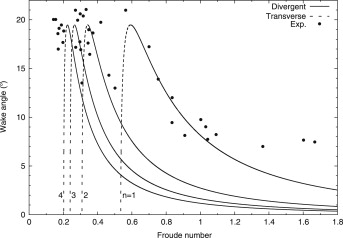
\includegraphics[width=0.5\textwidth]{chap3/psilongintrf.jpg}
  \bicaption[fig:psilongintrf]{单体船首尾波系干涉产生的波高最大的波的尾流角度}
  {单体船首尾散波(实线)或首尾横波(虚线)相长干涉造成的波高最大的波的尾流角度}{Fig}{Ray angles $\psi_n$ defined by \eqref{eq:psixn} with $1\le n\le 4$ along which divergent or transverse waves are
largest due to interference between the divergent (solid lines) or transverse
(dashed lines) waves created by the bow and the stern of a monohull ship}
\end{figure}

\section{双体船兴波特征}
\label{sec:catwavchar}

双体船两片体间距$s$在波浪传播方向$(\cos\gamma,\sin\gamma)$上的投影长度为
$s\sin\gamma$。由两片体首部产生的横波或散波间的相长干涉的发生条件为
\begin{equation}
  s\sin\gamma=n\lambda\equiv 2n\pi F^2\cos^2\gamma,\quad n\ge 1
  \label{eq:yunfavorintrf}
\end{equation}
由干涉条件\eqref{eq:yunfavorintrf}和式\eqref{eq:Fsdef}得
$\tan\gamma/\cos\gamma=2n\pi F_s^2$或者
\begin{equation}
  (1+\tan^2\gamma)\tan^2\gamma=4n^2\pi^2F_s^4
  \label{eq:yintrfrelation}
\end{equation}
由式\eqref{eq:yintrfrelation}和驻相关系\eqref{eq:statfazploar}可知
\begin{equation}
  \tan\psi_n^y=\sqrt{\frac{\sqrt{1+16n^2\pi^2F_s^4}-1}{2+32n^2\pi^2F_s^4}}
  \label{eq:psiyn}
\end{equation}
当Froude数$F_s=F_n^y$时,$\psi_n^y$等于Kelvin角$\psi^K$
\begin{equation}
  F_n^y=\frac{3^{1/4}}{2\sqrt{n\pi}}
  \label{eq:Fsn}
\end{equation}
由\eqref{eq:Fsn}可知
\begin{equation}
  F_1^y\equiv F_s^y\approx 0.37,\quad F_2^y\approx0.26,\quad F_3^y\approx 0.214,
  \quad F_4^y\approx 0.19, \cdots
\end{equation}
横波的相长干涉对应$0<F_s\le F_n^y$,而散波的相长干涉对应$F_s\ge F_n^y$。

令式\eqref{eq:psiyn}中$n=1$得
\begin{equation}
  \tan\psi_{\max}^y=\sqrt{\frac{\sqrt{1+16\pi^2F_s^4}-1}{2+32\pi^2F_s^4}}
  \label{eq:psiymax}
\end{equation}

图\ref{fig:psilatintrf}是$1\le n\le4$时双体船两片体产生的首波间相长干涉
造成的最大波高的尾流角度$\psi_n^y$,由式\eqref{eq:psiyn}定义。
其中,由横波和散波造成的干涉分别用虚线和实线表示。图中实线和虚线的连接点处
最大波高位于Kelvin臂上,其对应的Froude数由式\eqref{eq:Fsn}定义。图中还显示了
\parencite{Rabaud2013Ship}报告的处于$1.3<F<1.8$的观测数据。图\ref{fig:psilatintrf}
的横坐标是$F_s=F/\sqrt{s}$,而\parencite{Rabaud2013Ship}并未给出与观测数据对应的
船是单体船还是双体船。为了进行对比,假定处于$1.3<F<1.8$范围内的船是双体船,且片体
间距为$s=1$。从图\ref{fig:psilatintrf}可见,$1.3<F<1.8$范围内的观测数据与
双体船两片体首部区域产生的散波间的相长干涉产生的最大波高的尾流角$\psi_{\max}^y$
一致。
%
\begin{figure}[htp]
  \centering
  \captionstyle{\centering}
  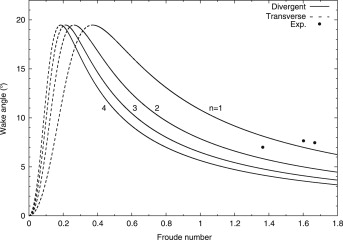
\includegraphics[width=0.5\textwidth]{chap3/psilatintrf.jpg}
  \bicaption[fig:psilatintrf]{双体船两片体首波系干涉产生的波高最大的波的尾流角度}
  {双体船两片体首部产生的散波(实线)或横波(虚线)干涉造成的波高最大的波的尾流
  角度}{Fig}
  {Ray angles $\psi_n^y$ defined by \eqref{eq:psiyn} with $1\le n\le 4$ 
  along which divergent or transverse waves are
largest due to interference between the divergent (solid lines) or transverse
(dashed lines) waves created by the bows of the twin hulls of a catamaran}
\end{figure}

\section{截断波长假设的逻辑漏洞}
\label{sec:cutoffwavlen}

由式\eqref{eq:disperploar}给出的色散关系$F^2k=1/\cos^2\gamma$可知波长
$\lambda=2\pi/k$可以表示为
\begin{equation}
  \lambda=2\pi F^2\cos^2\gamma\le 2\pi F^2\equiv \lambda^{\max}
  \label{eq:wavlenchap3}
\end{equation}
因此,船产生的最大波长$\lambda^{\max}$在$F<1/\sqrt{2\pi}\approx0.4$时小于船长,
在$F>0.4$时大于船长,正如众所周知的和第?章给出的。

由驻相关系\eqref{eq:disperploar}和式\eqref{eq:wavlenchap3}可知波长为$\lambda$
的尾流角度$\psi$是
\begin{equation}
  \tan\psi=\frac{\sqrt{\lambda^{max}/\lambda}-1}{2\lambda^{max}/\lambda-1}
  \equiv\frac{\sqrt{\lambda'(1-\lambda')}}{2-\lambda'}
  \quad\text{其中}\quad \lambda'=\lambda/\lambda^{\max}
  \label{eq:psiwavlen}
\end{equation}
由式\eqref{eq:psiwavlen}定义的$\psi$对$0\le\lambda'\le1$是实数。
当$0\le\lambda'\le2/3$时$\psi$从0增加到$\psi^K$,而当$2/3\le\lambda'\le1$时
$\psi$从$\psi^K$减小到0,如图\ref{fig:psiwavlen}所示。短波$0\le\lambda'\le 2/3$
和长波$2/3\le\lambda'\le 1$分别对应Kelvin波系中的散波和横波。
%
\begin{figure}[htp]
  \centering
  \captionstyle{\centering}
  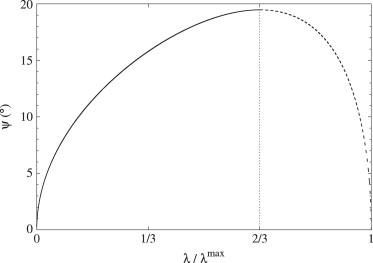
\includegraphics[width=0.5\textwidth]{chap3/psiwavlen.jpg}
  \bicaption[fig:psiwavlen]{尾流角度$\psi$随$\lambda/\lambda^{\max}$的变化}
  {当波长在$0\le\lambda/\lambda^{\max}\le1$范围内变化时,对应的尾流角度的变化}{Fig}
  {Variation of the corresponding ray angle $\psi$ for $0\le\lambda/\lambda^{\max}
\le1$}
\end{figure}

位于Kelvin臂$\psi=\psi^K$的波浪的波长为
\begin{equation}
  \lambda^{cusp}=2\lambda^{\max}/3=4\pi F^2/3
  \label{eq:wavlencusp}
\end{equation}
由式\eqref{eq:wavlencusp}可见,当$F<\sqrt{3/\pi}/2\approx0.49$时,Kelvin臂处的波长
$\lambda^{cusp}$小于船长,而当$F>0.49$时则大于船长。
现在我们只考虑$0\le\lambda\le\lambda^{cusp}$范围内的波浪,即散波。
由式\eqref{eq:psiwavlen}可知,尾流角度$\psi$上的散波的波长$\lambda^D$为
\begin{equation}
  \frac{\lambda^D}{\lambda^{\max}}}\equiv\frac{8\tan^2\psi}{1+4\tan^2\psi+
    \sqrt{1-8\tan^2\psi}}
  \label{eq:wavlendiv}
\end{equation}

对于散波$0\le\lambda\le\lambda^{cusp}$来说,由式\eqref{eq:psiwavlen}定义的函数
$\psi(\lambda)$是增函数。因此下面的不等式
\begin{eqnarray}
  &&\lambda\le\lambda^{cut}\quad\text{和} \label{eq:wavlenneq}\\
  &&\psi\le\psi^{cut}\equiv\arctan\left(
  \frac{\sqrt{\lambda^{max}/\lambda^{cut}-1}}{2\lambda^{max}/\lambda^{cut}-1}
  \right)
  \label{eq:psineq}
\end{eqnarray}
在数学上是等价的,其中$\lambda^{cut}\le\lambda^{cusp}$,$\psi^{cut}\le\psi^K$。
令式\eqref{eq:psineq}中$\lambda^{cut}=1$,即假设船波的波长不超过船长\supercite{Rabaud2013Ship},并将$\lambda^{\max}=2\pi F^2$代入,可得
\begin{equation}
  \tan\psi_{\max}=\frac{\sqrt{2\pi F^2-1}}{4\pi F^2-1}
  \label{eq:rabaudformula}
\end{equation}
式\eqref{eq:rabaudformula}即是\parencite{Rabaud2013Ship}预报的窄V字形尾迹的半角。

式\eqref{eq:wavlenneq}和式\eqref{eq:psineq}在数学上是等价的这一事实意味着,
假定$\lambda<\lambda^{cut}$也就自动将兴波角度$\psi$限制在Kelvin角$\psi^K$内,
因此无异于强制要求$\psi^{cut}\le\psi^K$。显然,引入截断波长假定的模型
(如\parencite{Rabaud2013Ship})无法解释观测到的窄V字形尾迹,除非假定的截断波长
$\lambda^{cut}$能够被证明是合理的。


\section{与最大波高对应的波长}
\label{sec:wavlen}

基于单体船首尾波系的相长干涉或双体船片体间首波系的相长干涉可以给出截断波长
$\lambda^{cut}$的一个合理定义。由前面的分析可知,单体船首尾散波系的相长干涉
会在尾流角度$\psi^x_{\max}$处产生波高最大的波,而双体船片体间首波系的相长干涉
会在尾流角度$\psi^y_{\max}$处产生波高最大的波。尾流角度$\psi^x_{\max}$和
$\psi^y_{\max}$分别由式\eqref{eq:psixmax}和\eqref{eq:psiymax}给出。
在$\psi^x_{\max}\le\psi\le\psi^K$或$\psi^y_{\max}\le\psi\le\psi^K$范围内的波浪
受干涉作用影响,波高小于$\psi^x_{\max}$或$\psi^y_{\max}$上波浪的波高,而由散波
波长$\lambda^D$和尾流角度$\psi$的关系可知,这些范围内的波浪波长大于$\psi^x_{\max}$
或$\psi^y_{\max}$上的波长。 因此波浪干涉作用抑制了波长大的散波的波高。
令式\eqref{eq:wavlendiv}中$\psi=\psi_{\max}$,得到对应$\psi_{\max}$和
基于波浪干涉作用的截断波长$\lambda^{cut}$
\begin{equation}
  \lambda^{cut}\equiv\frac{16\pi F^2\tan^2\psi_{max}}{1+4\tan^2\psi_{\max}+\sqrt{1-8\tan^2\psi_{\max}}}\approx 8\pi F^2\tan^2\psi_{\max}
  \label{eq:wavlencut}
\end{equation}

与单体船首尾波系的干涉和$\psi^x_{\max}$对应的截断波长可由\eqref{eq:psixmax}
和\eqref{eq:wavlencut}求得。由\eqref{eq:psixmax}和\eqref{eq:wavlencut}可知,
当$F\to\infty$时$\lambda^{cut}$的衰减形式为$1/F^2$。

与双体船片体间首波系的干涉和$\psi^y_{\max}$对应得截断波长可由\eqref{eq:psiymax}
和\eqref{eq:wavlencut}求得。由\eqref{eq:psiymax}和\eqref{eq:wavlencut}可知,
当$F\to\infty$时$\lambda^{cut}\to s$。

图\ref{fig:wavlencut}显示了单体船和片体间距为$s=0.1$,0.5,1和1.5的双体船对应的
截断波长$\lambda^{cut}$。当Froude数$F>1.2$时,双体船的截断波长几乎不随$F$变化,
且可以近似为$\lambda^{cut}\approx s$。
因此,假定截断波长是不随Froude变化的常数对双体船而言是合理的。
单体船的截断波长$\lambda^{cut}$是随Froude数$F$迅速衰减的函数,
因此,假定单体船的截断波长是不随Froude数变化的常数是不合理的。
所以,\parencite{Rabaud2013Ship}中的关键性假设$\lambda\le1$不能通过基于波浪干涉
的两点兴波模型得到的结果合理化。
%
\begin{figure}[htp]
  \centering
  \captionstyle{\centering}
  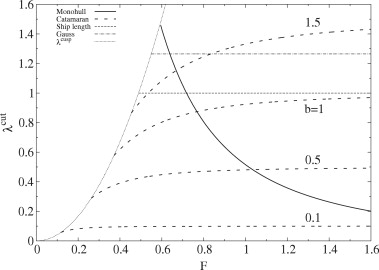
\includegraphics[width=0.5\textwidth]{chap3/wavlencut.jpg}
  \bicaption[fig:wavlencut]
  {单体船和双体船截断波长的变化}
  {与单体船首尾波系干涉和$s=0.1$,0.5,1和1.5的双体船片体间首波系干涉相关的
    截断波长$\lambda^{cut}$随Froude数$F$的变化}
  {Fig}{Variations of the cutoff wavelengths $\lambda^{cut}$ related to
  longitudinal interference between the divergent waves created by the bow
  and the stern of a monohull ship (Monohull) or to lateral interference
  between the divergent waves created by the twin hulls of a catamaran (catamaran)
with $s=0.1$, 0.5, 1 and 1.5}
\end{figure}


\section{本章小结}
\label{sec:analyssum}
本章首先总结了基于波浪干涉效应的两点兴波模型的分析。
由两点兴波模型预测的单体船首波和尾波间的相长干涉或双体船两片体产生的首波间的相长
干涉造成的波高最大的波浪的尾流角度与\parencite{Rabaud2013Ship}观测到的窄V字形尾迹
的半角一致。具体来说,图\ref{fig:psilongintrf}和图\ref{fig:psilatintrf}表明
\parencite{Rabaud2013Ship}的观测数据中Froude数小于或大于1.2的兴波角度分别与
单体船或双体船波高最大的波浪的尾流角度一致。因此波浪干涉是解释窄V字形船尾迹的
可信理论。
本章接着在线性势流理论的框架下对\parencite{Rabaud2013Ship}提出的截断波长假设
进行了批判性的分析。图\ref{fig:wavlencut}表明,截断波长$\lambda^{cut}$
与Froude数无关并约等于船长的假设\supercite{Rabaud2013Ship}无法用基于波浪干涉效应的
两点兴波模型\supercite{Noblesse2014Why}的分析合理化。

%%%# -*- coding: utf-8-unix -*-
\chapter{船舶兴波流动势的计算方法}
\label{chap:fsG}

\section{基本边界积分表达式}
\label{sec:bdryint}
考虑被封闭表面$\Sigma$包围的有限三维区域$\mathcal{D}$。域内或边界面上的点
为$\bm{\xi}\equiv(\xi,\eta,\zeta)$,点$\bm{\xi}\in\Sigma$处
垂直于表面$\Sigma$并指向域内的单位法向量为
$\mathbf{n}\equiv\mathbf{n}(\bm{\xi})$。

考虑定义在$\bm{\xi}\in\mathcal{D}\bigcup\Sigma$上的可微标量场
$\phi(\bm{\xi})$和$\psi(\bm{\xi})$。由Green第二公式得
\begin{equation}
  \int_\mathcal{D}\mathrm{d}v\,(\phi\nabla^2_\mathbf{\xi}\psi
  -\psi\nabla^2_{\mathbf{\xi}}\phi)
  =\int_\Sigma\mathrm{d}a\,\mathbf{n}\cdot(
  \psi\nabla_\mathbf{\xi}\phi
  -\phi\nabla_\mathbf{\xi}\psi
  )
  \label{eq:greentheorem}
\end{equation}
此处,$\nabla_\bm{\xi}$和$\nabla^2_\bm{\xi}$为
\begin{eqnarray}
  &\nabla_\mathbf{\xi}\equiv(\frac{\partial}{\partial\xi},
  \frac{\partial}{\partial\eta},\frac{\partial}{\partial\zeta})
  \label{eq:diff}\\
  &\nabla^2_\mathbf{\xi}\equiv\nabla_\mathbf{\xi}\cdot\mathbf{\xi}
  \equiv\frac{\partial^2}{\partial\xi^2}+\frac{\partial^2}{\partial\eta^2}
  +\frac{\partial^2}{\partial\zeta^2}\label{eq:laplace}
\end{eqnarray}
$\mathrm{d}v\equiv \mathrm{d}(\xi)$和$\mathrm{d}a=\mathrm{d}a(\xi)$是点
$\bm{\xi}\in\mathcal{D}$或$\bm{\xi}\in\Sigma$处的体积微元和面积微元。

取$\phi$为速度势,$\psi=G(\mathbf{x},\bm{\xi})$,这里
$G(\mathbf{x},\bm{\xi})$称作Green函数,满足Poisson方程
\begin{equation}
  \nabla^2_\mathbf{\xi}G=\delta(\xi-x)\delta(\eta-y)\delta(\zeta-z)
  \label{eq:Gdef}
\end{equation}
这里$\delta(\xi-x)$、$\delta(\eta-y)$、$\delta(\zeta-z)$是Dirac函数。
由$\nabla^2_{\bm{\xi}}\phi=0$、\eqref{eq:greentheorem}、\eqref{eq:Gdef}和
Dirac函数的性质得
\begin{eqnarray}
  \widetilde{C}\widetilde{\phi}=
  \int_\Sigma\mathrm{d}a\,(
  G\mathbf{n}\cdot\nabla_\mathbf{\xi}\phi
  -\phi\mathbf{n}\cdot\nabla_\mathbf{\xi}G
  )
  \label{eq:bdryint}
\end{eqnarray}
这里$\widetilde{\phi}\equiv\phi(\mahbf{x})$,当$\mathbf{x}\in\mathcal{D}$时取
$\widetilde{C}=1$,
当$\mathbf{x}\in\Sigma$时取$\widetilde{C}=1/2$,当$\mathbf{x}\notin\mathcal{D}$时取$\widetilde{C}=0$。当$\mathbf{x}\in\Sigma$时,表达式\eqref{eq:bdryint}只包含
$\phi$和它的法向导数$\mathbf{n}\cdot\nabla_{\bm{\xi}}\phi$在边界$\Sigma$上的值,
因此提供了确定$\phi$在边界$\Sigma$上值的(积分)方程。

式\eqref{eq:bdryint}将三维区域内点$\mathbf{x}$处的速度势$\phi(\mathbf{x})$
用$\phi(\mathbf{x})$和它的法向导数$\mathbf{n}\cdot\nabla_{\bm{\xi}}\phi=
\partial\phi/\partial n$在表面$\Sigma$上的值表示。因此,边界积分表达式
\eqref{eq:bdryint}将问题从三维降为二维。

\section{基本Green函数}
\label{sec:rankinesource}

满足Poisson方程\eqref{eq:Gdef}的一个Green函数是
\begin{equation}
  4\pi G=-1/r
  \label{eq:rankinesource}
\end{equation}
这里
\begin{equation}
  r\equiv\sqrt{(x-\xi)^2+(y-\eta)^2+(z-\zeta)^2}
  \label{eq:r}
\end{equation}
是点$\mathbf{x}=(x,y,z)$到点$\bm{\xi}=(\xi,\eta,\zeta)$之间的距离。
可以验证,$G$满足
\begin{equation}
  \nabla^2_{\bm{\xi}}G=0\quad\text{如果}\quad r>0
  \label{eq:laplaceG}
\end{equation}
与\eqref{eq:Gdef}一致。

注意到Green函数\eqref{eq:rankinesource}即满足Poisson方程\eqref{eq:Gdef}也满足如下
的Poisson方程
\begin{equation}
  \nabla^2_{\mathbf{x}}G\equiv(\partial^2/\partial x^2+\partial^2/\partial y^2
  +\partial^2/\partial z^2)G=\delta(x-\xi)\delta(y-\eta)\delta(z-\zeta)
  \label{eq:Gphyintrp}
\end{equation}
这表明Green函数\eqref{eq:rankinesource}可以看作位于点$\bm{\xi}$的单位点源在
场点$\mathbf{x}$处产生的速度势。
这种将$\mathbf{x}$看作场点和将$\bm{\xi}$看作源点的理解通常被采用。这表明
由边界积分表达式\eqref{eq:bdryint}定义的域$\mathcal{D}$内或边界面$\Sigma$上的
调和函数$\phi(\mathbf{x})$可以用分布在边界面$\Sigma$上的点源$G$和偶极子$\mathbf{n}\cdot\nabla_{\bm{\xi}}G$表示,并且点源和偶极子的强度分别等于$\mathbf{n}\cdot\nabla_{\bf{\xi}}\phi$和$\phi$。



\section{自由面Green函数}
\label{sec:fsG}

满足Poisson方程\eqref{eq:Gdef}的Green函数不是唯一的。事实上,任何形如
\begin{equation}
  4\pi G=-1/r+H,\quad\text{其中}\quad \nabla^2_{\bm{\xi}}H=0,\quad\text{对于}
  \quad\bm{\xi}\in\mathcal{D}
  \label{eq:generalG}
\end{equation}
的Green函数都满足Poisson方程\eqref{eq:Gdef}。

对于船在无限深广的静水中匀速前进的问题,边界积分表达式中的积分边界$\Sigma$
可取为
\begin{equation}
  \Sigma=\Sigma^H+\Sigma^F+\Sigma^\infty
  \label{eq:bdry}
\end{equation}
其中$\Sigma_a^H$代表平均船体湿表面,$\Sigma^F$代表位于船体表面外的平均自由面,
$\Sigma^\infty$代表包含流场$\mathcal{D}$的半径趋于无穷大的下半球面。

我们在第?章推导了船在无限深广的静水中匀速前进的速度势$\phi$满足的定解条件。
为了方便本章应用,现重新列出如下
\begin{subequations}\label{eq:govreiter}
  \begin{eqnarray}
  &&\nabla^2_{\bm{\xi}}\phi\equiv
  (\partial^2/\partial\xi^2+\partial^2/\partial\eta^2+\partial^2/\partial\zeta^2)\phi=0,\quad \bm{\xi}\in\mathcal{D}\label{eq:govreiter-a}\\
  &&[\partial/\partial\zeta+(F\partial/\partial\xi-\epsilon)^2]\phi=0,\quad\bm{\xi}
  \in\Sigma^{F}\label{eq:govreiter-fs}\\
  &&\mathbf{n}\cdot\nabla_{\bf{\xi}}\phi=n_x, \quad \bm{\xi}\in\Sigma^H
  \label{eq:govreiter-hull}\\
  &&\phi\rightarrow0, \quad \bm{\xi}\in\Sigma^\infty
  \label{eq:govreiter-far}
\end{eqnarray}
\end{subequations}

当$r\to\infty$时,基本Green函数\eqref{eq:rankinesource}的量阶是$\mathcal{O}(1/r)$.
而$\mathbf{n}\cdot\nabla_{\bm{\xi}}\phi$的量阶是$\mathcal{O}(\phi/r)$,因此
$G\mathbf{n}\cdot\nabla_{\bm{\xi}}\phi$的量阶是$\mathcal{O}(\phi/r^2)$。
同理可知,基本边界积分表达式\eqref{eq:bdryint}中整个被积函数的量阶为
$\mathcal{O}(\phi/r^2)$。无穷远表面积的量纲是$\mathcal{O}(r^2)$。
由此可知当$r\to\infty$时,边界积分表达式\eqref{eq:bdryint}在$\Sigma^\infty$的
积分值为零。

由边界积分表达式\eqref{eq:bdryint}、积分边界\eqref{eq:bdry}、
速度势船体表面边界条件\eqref{eq:govreiter-hull},考虑远场$\Sigma^{\infty}$对
边界积分表达式\eqref{eq:bdryint}的影响得
\begin{equation}
  \tilde\phi=\int_{\Sigma^H}(Gn^x-\phi\mathbf{n}\cdot\nabla G)\,\mathrm{d}a
  +\int_{\Sigma^F}(\phi G_{\zeta}-G\phi_{\zeta})\,\mathrm{d}\xi\mathrm{d}\eta
  \label{eq:bdryintmean}
\end{equation}

如果我们选择的Green函数满足如下齐次自由面边界条件
\begin{equation}
  [\partial/\partial\zeta+(\epsilon+F\partial/\partial\xi)^2]G=0, \quad \zeta=0
  \label{eq:Gbdry-fs}
\end{equation}
则由式\eqref{eq:govreiter-fs}、\eqref{eq:Gbdry-fs}可知
\begin{equation}
  \phi G_{\zeta}-\G\phi_{\zeta}=F^2(G\phi_{\xi}-\phi G_{\xi})_{\xi}
  \label{eq:fsintegrand}
\end{equation}
由此可知
\begin{eqnarray}
  \int_{\Sigma^F}\mathrm{d}\xi\mathrm{d}\eta\,
  (\phi G_{\zeta}-G\phi_{\zeta})
  &=&F^2\int_{\Gamma}(G\phi_\xi-\phi G_\xi)\,\mathrm{d}\eta \nonumber\\
  &=&F^2\int_{\Gamma}(G\phi_{\xi}-\phi G_{\xi})t^y\mathrm{d}\ell
  \label{eq:watr}
\end{eqnarray}
这里使用了Stokes定理将在自由面$\Sigma^F$上的积分转化为在平均水线$\Gamma$上的线积分。
这里水线$\Gamma$的方向(从上往下看)为顺时针方向,$\mathrm{d}\ell$是水线$\Gamma$的
弧长微元,$\mathbf{t}\equiv (t^x,t^y,0)$是水线$\Gamma$的单位切向量。
因此在左舷$y\ge0$,$\mathbf{t}$指向船首,我们有$\mathbf{t}=(n^y,-n^x,0)/\sqrt{(n^x)^2+(n^y)^2}$,其中$\mathbf{n}=(n^x,n^y,n^z)$是船体曲面的外法向量(指向水中)。


通过选择\eqref{eq:generalG}中调和函数$H$,可使Green函数$G$满足自由面边界条件
\eqref{eq:Gbdry-fs}。此Green函数还满足下半平面$\zeta<0$内的Poisson方程
\eqref{eq:Gdef}和无穷远条件:当$r\to\infty$时,$G\to0$。
因此Green函数$G(\mathbf{x},\bm{\xi})$是下述问题的解
\begin{subequations}\label{eq:Gbdry}
  \begin{eqnarray}
    &&\Delta^2_{\bm{\xi}}G=\delta(\xi-x)\delta(\eta-y)\delta(\zeta-z),\quad \zeta<0
    \label{eq:Gbdrygov}\\
    &&G\to0,\quad r\to\infty\label{eq:Gbdryfar}\\
    &&[\partial/\partial\zeta+(\epsilon+F\partial/\partial\xi)^2]G=0,\quad \zeta=0
    \label{eq:Gbdryfs}
  \end{eqnarray}
\end{subequations}

满足问题\eqref{eq:Gbdry}的一般解为
\begin{equation}
  4\pi G=-1/r+1/r'+P/\pi
  \label{eq:fsGgeneral}
\end{equation}
这里
\begin{equation}
  r'=\sqrt{(x-\xi)^2+(y-\eta)^2+(z-\zeta)^2}
  \label{eq:r'}
\end{equation}
是点$\bm{\xi}=(\xi,\eta,\zeta)$到点$\mathbf{x}=(x,y,z)$关于自由面$\zeta=0$的镜像
$\mathbf{x'}=(x,y,-z)$的距离。函数$1/r'$满足下半平面$\zeta<0$内的Laplace方程。

函数$P$是下述问题的解
\begin{subequations}\label{eq:Pbdry}
  \begin{eqnarray}
    &&\nabla^2_{\bm{\xi}}P=0,\quad \zeta<0\label{eq:Pbdrygov}\\
    &&P\to 0,\quad r\to\infty\label{eq:Pbdryfar}\\
    &&[\partial/\partial\zeta+(\epsilon+F\partial/\partial\xi)^2]P
    =-2\pi\partial(1/r')/\partial\zeta,\quad \zeta=0
    \label{eq:Pbdryfs}
  \end{eqnarray}
\end{subequations}
式\eqref{eq:fsGgeneral}将Green函数分为基本Green函数$-1/r$和另外两部分的和。
$1/r'$对应于将自由面边界条件取为$G=0$,这相当于在\eqref{eq:Gbdryfs}中$F\to\infty$。
$P$考虑了自由面边界的效应。

由边界条件\eqref{eq:Pbdryfs}和式\eqref{eq:r'}可得,调和函数$P$只依赖于
\begin{equation}
  x-\xi,\quad y-\eta,\quad z+\zeta
  \label{eq:3var}
\end{equation}
三个变量。
另外,由式\eqref{eq:fsGgeneral}可知在自由面$\zeta=0$上$r=r'$,因此Green函数只依赖于
变量$x-\xi$,$y-\eta$,$z+\zeta$。因此,自由面条件\eqref{eq:Gbdryfs}也可以写作
如下等价形式
\begin{equation}
  [\partial/\partial z+(F\partial/\partial x-\epsilon)^2]G=0
  \label{eq:Gbdryfs-b}
\end{equation}
而Poisson方程\eqref{eq:Gbdrygov}也可表示成等价形式\eqref{eq:Gphyintrp}。
因此Green函数也是下述问题的解
\begin{subequations}\label{eq:fsG}
  \begin{eqnarray}
    && (\partial^2/\partial x^2+\partial^2/\partial y^2+\partial^2/\partial z^2)G=\delta(x-\xi)\delta(y-\eta)\delta(z-\zeta),\quad z<0
    \label{eq:fsGgov}\\
  &&[\partial/\partial z+(F\partial/\partial x-\epsilon)^2]G=0,\quad z=0
  \label{eq:fsGfs}\\
  && G\to\infty,\quad r\to\infty \label{eq:fsGfar}
  \end{eqnarray}
\end{subequations}

式\eqref{eq:fsG}表明,Green函数$G(\mathbf{x},\bm{\xi})$可看作存在自由面时,
位于$\bf{\xi}$的点源在场点$\mathbf{x}$处产生的速度势。

\section{双重积分形式Green函数}
\label{sec:fsGiint}

下面求解满足\eqref{eq:Gbdry}的Green函数。此Green函数的形式为\eqref{eq:fsGgeneral},
其中函数$P$是满足\eqref{eq:Pbdry}的解。通过对坐标$\xi$和$\eta$进行双Fourier变换
可求得函数$P$。

记$1/r$的Fourier变换为$(1/r)^*$。
考虑到$1/r$满足Poisson方程,即
\begin{equation}
  (\partial^2/\partial\xi^2+\partial^2/\partial\eta^2+\partial^2/\partial\zeta^2)
  (1/r)=-4\pi\delta(\xi-x)\delta(\eta-y)\delta(\zeta-z)
  \label{eq:req}
\end{equation}
对\eqref{eq:req}进行Fourier变换得
\begin{equation}
  \mathrm{d}^2(1/r)^*/\mathrm{d}\zeta^2-k^2(1/r)^*=-2\mathrm{e}^{-\mathrm{i}(\alpha x+\beta y)}\delta(\zeta-z)
  \label{eq:reqft}
\end{equation}
其中$k^2=\alpha^2+\beta^2$。微分方程\eqref{eq:reqft}的通解为
\begin{equation*}
  (1/r)^*=A^{+}\mathrm{e}^k\zeta+A^{-}\mathrm{e}^{-k\zeta}
\end{equation*}
其中$A^+$与$A^-$为常数。由于$1/r$是$\zeta-z$的偶函数,且当$\zeta-z\to\pm\infty$时
趋于零,所以$(1/r)^*$可表示为
\begin{equation}
  (1/r)^*=A\mathrm{e}^{-k|\zeta-z|}
  \label{eq:rftgen-b}
\end{equation}
其中$A$为未知常数。

由式\eqref{eq:rftgen-b}定义的函数$(1/r)^*$在$\zeta=z$处连续且等于$A$。
而它的导数在$\zeta=z$不连续。特别地,导数$\mathrm{d}(1/r)^*/\mathrm{d}\zeta)$为
\begin{equation*}
  \frac{\mathrm{d}(1/r)^*}{\mathrm{d}\zeta}=
  \left\{
    \begin{array}{ll}
      kA\mathrm{e}^{k(\zeta-z)}, & \zeta<z \\
      -kA\mathrm{e}^{-k(\zeta-z)}, & z<\zeta
    \end{array}
    \right.
\end{equation*}
由此可知
\begin{equation}
  \frac{\mathrm{d}(1/r)^*}{\mathrm{d}\zeta}=
  \left\{
    \begin{array}{ll}
      kA, & \zeta=z-0 \\
      -kA, & \zeta=z+0
    \end{array}
    \right.
  \label{eq:drdzcoin}
\end{equation}
将式\eqref{eq:reqft}对$\zeta$在区间$[z-0,z+0]$进行积分得
\begin{equation*}
  [\mathrm{d}(1/r)^*/\mathrm{d}\zeta]|^{z+0}_{z-0}-k^2\int_{z-0}^{z+0}
  \mathrm{d}\zeta\,(1/r)^*=-2\mathrm{e}^{-\mathrm{i}(\alpha x+\beta y)}
\end{equation*}
由此式和式\eqref{eq:drdzcoin}可得
$-2kA=-2\mathrm{e}^{-\mathrm{i}(\alpha x+\beta y)}$。因此
\begin{equation*}
  A=\mathrm{e}^{-\mathrm{i}(\alpha x+\beta y)}/k
\end{equation*}
由此式和式\eqref{eq:rftgen-b}得
\begin{equation}
(1/r)^*=\mathrm{e}^{-k|z-\zeta|-\mathrm{i}(\alpha x+\beta y)}/k
  \label{eq:rft}
\end{equation}

考虑到$1/r'$是点$\bm{\xi}\equiv(\xi,\eta,\zeta)$到点$\mathbf{x}\equiv(x,y,z)$关于
$\zeta=0$的镜像点$\mathbf{x'}\equiv(x,y,-z)$的距离。在式\eqref{eq:rft}中将$z$
替换为$-z$并注意到$(z+\zeta)< 0$可得
\begin{equation}
  (1/r')^*=\mathrm{e}^{k(z+\zeta)-\mathrm{i}(\alpha x+\beta y)}/k,\quad z<0\quad\text{且}\quad\zeta<0
  \label{eq:r'ft}
\end{equation}

函数$P$的Fourier变换为
\begin{equation}
  P^*(\alpha,\beta,\zeta;\mathbf{x})=\frac{1}{2\pi}\int_{-\infty}^{\infty}
  \mathrm{d}\eta\int_{-\infty}^{\infty}\mathrm{d}\xi\,\mathrm{e}^{-\mathrm{i}(\alpha\xi+\beta\eta)}P(\xi,\eta,\zeta;\mathbf{x})
  \label{eq:Pfourier}
\end{equation}
其逆变换为
\begin{equation}
  P(\xi,\eta,\zeta;\mathbf{x}})=\frac{1}{2\pi}\int_{-\infty}^{\infty}
  \mathrm{d}\beta\int_{-\infty}^{\infty}\mathrm{d}\alpha\,\mathrm{e}^{\mathrm{i}(\alpha\xi+\beta\eta)}P^*(\alpha,\beta,\zeta;\mathbf{x})
  \label{eq:Pfourierinv}
\end{equation}

对\eqref{eq:Pbdry}进行Fourier变换可得
\begin{subequations}\label{eq:Peqft}
  \begin{eqnarray}
    && \mathrm{d}^2P^*/\mathrm{d}\zeta^2-k^2P^*=0,\quad -\infty<\zeta<0
    \label{eq:Peqftgov}\\
    && P^*\to 0,\quad \zeta\to -\infty\label{eq:Peqftfar}\\
    && \mathrm{d}P^*/\mathrm{d}\zeta-[F^2\alpha^2-2\mathrm{i}\epsilon F\alpha-\epsilon^2]P^*=-2\pi\mathrm{e}^{kz-\mathrm{i}(\alpha x+\beta y)},\quad \zeta=0
    \label{eq:Peqftfs}
  \end{eqnarray}
\end{subequations}
微分方程\eqref{eq:Peqft}的通解为
\begin{equation}
  P^*=A^{+}\mathrm{e}^{k\zeta}+A^{-}\mathrm{e}^{-k\zeta}
  \label{eq:Pftgen}
\end{equation}
其中$A^{+}$与$A^{-}$为常数。由边界条件\eqref{eq:Peqftfar}可知$A^{-}=0$。
由边界条件\eqref{eq:Peqftfs}可得解为
\begin{equation}
  P^*=2\pi\mathrm{e}^{k(z+\zeta)-\mathrm{i}(\alpha x+\beta y)}/[k-(F\alpha-\mathrm{i}\epsilon)^2]
  \label{eq:Pft}
\end{equation}
由\eqref{eq:Pfourierinv}得
\begin{equation}
  P=-\int_{-\infty}^{\infty}\mathrm{d}\beta\int_{-\infty}^{\infty}\mathrm{d}\alpha\,
  \frac{\mathrm{e}^{k(z+\zeta)-\mathrm{i}[\alpha(x-\xi)+\beta(y-\eta)]}}{k-(F\alpha-\mathrm{i}\epsilon)^2}
  \label{eq:Piint}
\end{equation}

由\eqref{eq:generalG}和式\eqref{eq:Piint}得
\begin{equation}
  4\pi G=\frac{-1}{r}+\frac{1}{r'}-\frac{1}{\pi}
  \int_{-\infty}^{\infty}\mathrm{d}\beta\int_{-\infty}^{\infty}\mathrm{d}\alpha\,
  \frac{\mathrm{e}^{k(z+\zeta)-\mathrm{i}[\alpha(x-\xi)+\beta(y-\eta)]}}{k-(F\alpha-\mathrm{i}\epsilon)^2}
  \label{eq:Giint}
\end{equation}
这是双重积分形式的线性自由表面兴波Green函数。但由于累次积分形式Green函数难于处理,
下面将给出单重积分形式的Green函数,以便于分析和数值计算。

\section{单重积分形式Green函数}
\label{sec:Gint}

记$x'=x-\xi$,$y'=y-\eta$,$z'=z+\zeta$,双重积分形式Green函数\eqref{eq:Giint}
可改写为
\begin{equation}
  4\pi G=\frac{-1}{r}+\frac{1}{r'}-\frac{1}{\pi}\int_{-\infty}^{\infty}
  \mathrm{e}^{-\mathrm{i}y'\beta}I_1(\beta,x',z',\epsilon)\,\mathrm{d}\beta
  \label{eq:inti1}
\end{equation}
其中,$I_1$为
\begin{equation}
  I_1(\beta;x',z',\epsilon)=\int_{-\infty}^{\infty}
  \frac{\mathrm{e}^{\sqrt{\alpha^2+\beta^2}z'-\mathrm{i}\alpha x'}}{\sqrt{\alpha^2+\beta^2}-(\alpha-\mathrm{i}\epsilon)^2}\,
  \mathrm{d}\alpha
  \label{eq:I1}
\end{equation}

$I_1$的被积函数有两个一阶极点,它们是方程
$\sqrt{\alpha^2+\beta^2}=(\alpha-\mathrm{i}\epsilon)^2$的根。
求解该方程可知当$\epsilon\to 0$时,两根为$\pm s+\mathrm{i}0$,即方程的根
从上半平面趋于$\pm s$。这里
\begin{equation}
  s=\sqrt{\frac{1+\sqrt{1+4\beta^2}}{2}}
  \label{eq:2poles}
\end{equation}
极点的位置在图\ref{fig:cntrint}中表出。可把积分$I_1$看作包含实轴的围道积分在实轴上的积分。
由于$\sqrt{\alpha^2+\beta^2}$是$\alpha$平面上的多值函数,其支点为
$\alpha=\pm\mathrm{i}|\beta|$,为了得到单值分支,需要将$\alpha$平面沿支割线
割破。这里支割线选为$\alpha=\mathrm{i}\alpha_i$,其中$-\infty<\alpha_i<-|\beta|$
或$|\beta|<\alpha_i<\infty$,对应于将复变函数$\sqrt{z}$的支割线选为$z<0$。
支割线的位置在图\ref{fig:cntrint}中表出。
要使用围道积分,需满足条件
\begin{equation*}
  \mathrm{Re}[z'\sqrt{\alpha^2+\beta^2}-\mathrm{i}x'\alpha]\le 0,
  \quad |\alpha|\to\infty
\end{equation*}
此时显然有
\begin{equation}
  \lim_{|\alpha|\to\infty}\frac{\alpha\mathrm{e}^{\sqrt{\alpha^2+\beta^2}z'-\mathrm{i}\alpha x'}}{\sqrt{\alpha^2+\beta^2}-(\alpha-\mathrm{i}\epsilon)^2}=0
  \label{eq:intcntr}
\end{equation}
可以验证,图\ref{fig:cntrint}所示的围道积分满足该条件。
\begin{figure}[htp]
  \centering
  \captionstyle{\centering}
  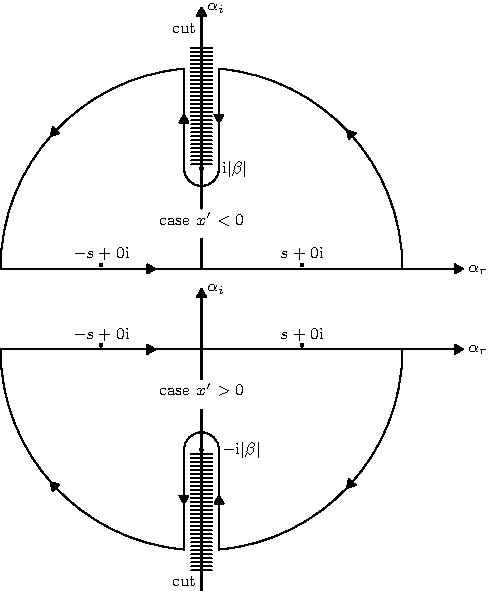
\includegraphics[width=0.5\textwidth]{chap4/contour_int.pdf}
  \bicaption[fig:cntrint]{复平面$\alpha=\alpha_r+\mathrm{i}\alpha_i$上的积分围道}
  {复平面$\alpha=\alpha_r+\mathrm{i}\alpha_i$上当$x'<0$和$x'>0$时的积分围道}{Fig}
  {Integration contours in the complex $\alpha=\alpha_r+\mathrm{i}\alpha_i$
plane for $x'<0$ and $x'>0$}
\end{figure}

首先考虑$x'>0$的情形。在支割线$\alpha_r=0,-\infty<\alpha_i<-|\beta|$的两边
$\alpha=\pm 0+\mathrm{i}\alpha_i$,我们有$\sqrt{\alpha^2+\beta^2}=\mp\mathrm{i}\sqrt{\alpha_i^2-\beta^2}$。在对应$x'>0$的围道内被积函数解析,考虑到式\eqref{eq:intcntr}
,由Cauchy积分定理得
\begin{equation*}
  I_1+\int_{-\infty}^{-|\beta|}
  \frac{\mathrm{e}^{\alpha_i x'-\mathrm{i}\sqrt{\alpha_i^2-\beta^2}z'}}{\alpha_i^2-
    \mathrm{i}\sqrt{\alpha_i^2-\beta^2}}\mathrm{i}\,\mathrm{d}\alpha_i
  +\int_{-|\beta|}^{-\infty}
  \frac{\mathrm{e}^{\alpha_i x'+\mathrm{i}\sqrt{\alpha_i^2-\beta^2}z'}}{\alpha_i^2+
    \mathrm{i}\sqrt{\alpha_i^2-\beta^2}}\mathrm{i}\,\mathrm{d}\alpha_i=0
\end{equation*}
将上式两个积分项移到等式右边,整理得
\begin{equation*}
  I_1=\int_{-\infty}^{-|\beta|}
  \frac{\mathrm{e}^{\alpha_i x'+\mathrm{i}\sqrt{\alpha_i^2-\beta^2}z'}}{\alpha_i^2+
    \mathrm{i}\sqrt{\alpha_i^2-\beta^2}}\mathrm{i}\,\mathrm{d}\alpha_i
  +\int_{-|\beta|}^{-\infty}
  \frac{\mathrm{e}^{\alpha_i x'-\mathrm{i}\sqrt{\alpha_i^2-\beta^2}z'}}{\alpha_i^2-
    \mathrm{i}\sqrt{\alpha_i^2-\beta^2}}\mathrm{i}\,\mathrm{d}\alpha_i
\end{equation*}
对上式第一个积分项和第二个积分项分别作变量代换$\mu=\sqrt{\alpha_i^2-\beta^2}$和
$\mu=-\sqrt{\alpha_i^2-\beta^2}$得
\begin{equation}
  I_1=\mathrm{i}\int_{-\infty}^{\infty}
  \frac{\mathrm{e}^{-x'\sqrt{\mu^2+\beta^2}+\mathrm{i}\mu z'}}{(\mu^2+\beta^2+\mathrm{i}\mu)\sqrt{\mu^2+\beta^2}}\mu\,\mathrm{d}\mu
  \label{eq:I1mu-a}
\end{equation}

下面考虑$x'<0$的情形。在支割线$\alpha_r=0,|\beta|<\alpha_i<\infty$的两边
$\alpha=\pm 0+\mathrm{i}\alpha_i$,
我们有$\sqrt{\alpha^2+\beta^2}=\pm\mathrm{i}\sqrt{\alpha_i^2-\beta^2}$。
在对应$x'<0$的围道内被积函数有两个一阶极点$\alpha=\pm s$,考虑到式\eqref{eq:intcntr}
,由留数定理得
\begin{equation*}
  I_1+\int_{\infty}^{|\beta|}
  \frac{\mathrm{e}^{\alpha_i x'+\mathrm{i}\sqrt{\alpha_i^2-\beta^2}z'}}{\alpha_i^2+
    \mathrm{i}\sqrt{\alpha_i^2-\beta^2}}\mathrm{i}\,\mathrm{d}\alpha_i
  +\int_{|\beta|}^{\infty}
  \frac{\mathrm{e}^{\alpha_i x'-\mathrm{i}\sqrt{\alpha_i^2-\beta^2}z'}}{\alpha_i^2-
    \mathrm{i}\sqrt{\alpha_i^2-\beta^2}}\mathrm{i}\,\mathrm{d}\alpha_i=
    2\pi\mathrm{i}[\mathrm{Res}(s)+\mathrm{Res}(-s)]
\end{equation*}
将上式左边两个积分项移到等式右边,整理后得
\begin{equation*}
  I_1=\int_{\infty}^{|\beta|}
  \frac{\mathrm{e}^{\alpha_i x'-\mathrm{i}\sqrt{\alpha_i^2-\beta^2}z'}}{\alpha_i^2-
    \mathrm{i}\sqrt{\alpha_i^2-\beta^2}}\mathrm{i}\,\mathrm{d}\alpha_i
  +\int_{|\beta|}^{\infty}
  \frac{\mathrm{e}^{\alpha_i x'+\mathrm{i}\sqrt{\alpha_i^2-\beta^2}z'}}{\alpha_i^2+
    \mathrm{i}\sqrt{\alpha_i^2-\beta^2}}\mathrm{i}\,\mathrm{d}\alpha_i+
    2\pi\mathrm{i}[\mathrm{Res}(s)+\mathrm{Res}(-s)]
\end{equation*}
其中$\mathrm{Res}(\pm s)$是被积函数在极点$\alpha=\pm s$的留数,我们有
\begin{equation*}
  \mathrm{Res}(\pm s)=\mp\frac{\mathrm{e}^{z'\sqrt{s^2+\beta^2}\mp\mathrm{i}sx'}}{2s-1/s}
\end{equation*}
类似于$x'>0$时的情形,再对上式第一个积分项和第二个积分项分别作变量代换
$\mu=-\sqrt{\alpha_i^2-\beta^2}$和$\mu=\sqrt{\alpha_i^2-\beta^2}$得
\begin{equation}
  I_1=\mathrm{i}\int_{-\infty}^{\infty}
  \frac{\mathrm{e}^{x'\sqrt{\mu^2+\beta^2}+\mathrm{i}\mu z'}}{(\mu^2+\beta^2+\mathrm{i}\mu)\sqrt{\mu^2+\beta^2}}\mu\,\mathrm{d}\mu-\frac{4\pi}{2s-1/s}\mathrm{e}^
  {z'\sqrt{s^2+\beta^2}}\sin(sx')
  \label{eq:I1mu-b}
\end{equation}

对比积分$I_1$在$x'>0$情形下的表达式\eqref{eq:I1mu-a}和在$x'<0$情形下的表达式
\eqref{eq:I1mu-b}可知$I_1$可表示成如下统一形式
\begin{equation}
  I_1=\mathrm{i}\int_{-\infty}^{\infty}
  \frac{\mathrm{e}^{-|x'|\sqrt{\mu^2+\beta^2}+\mathrm{i}\mu z'}}{(\mu^2+\beta^2+\mathrm{i}\mu)\sqrt{\mu^2+\beta^2}}\mu\,\mathrm{d}\mu-\frac{H(-x')4\pi}{2s-1/s}
  \mathrm{e}^{z'\sqrt{s^2+\beta^2}}\sin(sx')
  \label{eq:I1mu}
\end{equation}
将式\eqref{eq:I1mu}代回式\eqref{eq:inti1},整理得Green函数可表示成如下形式
\begin{equation}
  4\pi G(\mathbf{x};\bm{\xi})=-1/r+N_1(\mathbf{x'})+W_1(\mathbf{x'})
  \label{eq:Gnw}
\end{equation}
其中
\begin{eqnarray}
  && N_1(\mathbf{x'})=\frac{1}{r'}-\frac{\mathrm{i}}{\pi}\int_{-\infty}^{\infty}
  \mathrm{d}\beta\,\mathrm{e}^{-\mathrm{i}y'\beta}\int_{-\infty}^{\infty}
  \frac{\mathrm{e}^{-|x'|\sqrt{\mu^2+\beta^2}+\mathrm{i}\mu z'}}{(\mu^2+\beta^2+\mathrm{i}\mu)\sqrt{\mu^2+\beta^2}}\mu\,\mathrm{d}\mu \label{eq:N1}\\
  && W_1(\mathbf{x'})=H(-x')4\int_{-\infty}^{\infty}\frac{\mathrm{e}^{z'\sqrt{s^2+\beta^2}-\mathrm{i}y'\beta}}{2s-1/s}\sin(sx')\,\mathrm{d}\beta\label{eq:W1}
\end{eqnarray}
对式\eqref{eq:W1}作变量代换$\beta=t\sqrt{1+t^2}$得
\begin{equation*}
  W_1(\mathbf{x'})=H(-x')4\int_{-\infty}^{\infty}
  \mathrm{e}^{z'(1+t^2)-\mathrm{i}y't\sqrt{1+t^2}}\sin(x'\sqrt{1+t^2})\,
  \mathrm{d}t
\end{equation*}
注意到被积函数的奇偶性对积分的影响,有
\begin{equation}
  W_1(\mathbf{x'})=H(-x')4\int_{-\infty}^{\infty}\mathrm{Im}[
  \mathrm{e}^{z'(1+t^2)+\mathrm{i}(x'+y't)\sqrt{1+t^2}}]\,\mathrm{d}t
  \label{eq:W1im}
\end{equation}

下面考虑二重积分$N_1$。式\eqref{eq:N1}可以改写成如下形式
\begin{equation*}
  N_1(\mathbf{x'})=\frac{1}{r'}-\frac{\mathrm{i}}{\pi}\int_{-\infty}^{\infty}
  \int_{-\infty}^{\infty}\frac{\mathrm{e}^{-|x'|\sqrt{\mu^2+\beta^2}+\mathrm{i}(\beta y'+\mu z')}}{(\mu^2+\beta^2+\mathrm{i}\mu)\sqrt{\mu^2+\beta^2}}\mu\,
  \mathrm{d}\beta\mathrm{d}\mu
\end{equation*}
作坐标变换$\beta=\rho\cos\theta$,$\mu=\rho\sin\theta$,将直角坐标系$(\beta,\mu)$
转化为极坐标系$(\rho,\theta)$,可得
\begin{equation}
  N_1(\mathbf{x'})=\frac{1}{r'}-\frac{\mathrm{i}}{\pi}\int_{-\pi}^{\pi}
  I(\theta;\mathbf{x'})\sin\theta\,\mathrm{d}\theta
  \label{eq:N1polar}
\end{equation}
其中$I(\theta;\mathbf{x'})$由下式给出
\begin{equation*}
  I(\theta;\mathbf{x'})=\int_0^{\infty}\frac{\mathrm{e}^{-[|x'|-\mathrm{i}(y'\cos\theta+z'\sin\theta)]\rho}}{\rho+\mathrm{i}\sin\theta}\,\mathrm{d}\rho
\end{equation*}
作变量代换$\tau=\rho+\mathrm{i}\sin\theta$得
\begin{equation*}
  I(\theta;\mathbf{x'})=\mathrm{e}^\zeta\int_{\mathrm{i}\sin\theta}^{\infty}
  \mathrm{e}^{-[|x'|-\mathrm{i}(y'\cos\theta+z'\sin\theta)\tau]}\frac{\mathrm{d}\tau}{\tau}
\end{equation*}
这里$\zeta$是复变函数,为
\begin{equation}
  \zeta=(y'\cos\theta+z'\sin\theta+\mathrm{i}|x'|)\sin\theta
  \label{eq:zeta}
\end{equation}
作变量代换$\lambda=[|x'|-\mathrm{i}(y'\cos\theta+z'\sin\theta)]\tau$,我们有
\begin{equation}
  I(\theta;\mathbf{x'})=\mathrm{e}^\zeta\int_{\zeta}^{\infty}
  \mathrm{e}^{-\lambda}\frac{\mathrm{d}\lambda}{\lambda}=\mathrm{e}^\zeta E_1(\zeta)
  \label{eq:Izeta}
\end{equation}
其中$E_1(\zeta)$是复指数积分函数,取负半实轴为支割线。
将内部积分$I(\theta;\mathbf{x'})$的表达式\eqref{eq:Izeta}代入式\eqref{eq:N1polar}
得
\begin{eqnarray*}
  N_1(\mathbf{x'})&=&\frac{1}{r'}-\frac{\mathrm{i}}{\pi}\int_{\pi}^{\pi}
  \mathrm{e}^\zeta E_1(\zeta)\sin\theta\,\mathrm{d}\theta\\
  &=& \frac{1}{r'}-\frac{\mathrm{i}}{\pi}\left\{
  \int_0^\pi  
  \mathrm{e}^\zeta E_1(\zeta)\sin\theta\,\mathrm{d}\theta
  +\int_{-\pi}^0\mathrm{e}^\zeta E_1(\zeta)\sin\theta\,\mathrm{d}\theta
\right\}\\
&=&\frac{1}{r'}-\frac{\mathrm{i}}{\pi}\left\{
  \int_0^\pi  
  \mathrm{e}^\zeta E_1(\zeta)\sin\theta\,\mathrm{d}\theta
  -\int_0^\pi\mathrm{e}^{\bar{\zeta} E_1(\bar{\zeta})}\sin\psi\,\mathrm{d}\psi
\right\}
\end{eqnarray*}
这里使用了变量代换$\psi=\theta+\pi$,$\bar{\zeta}$是由\eqref{eq:zeta}定义的
复变函数$\zeta$的复共轭函数。由关系式$\exp(\bar{\zeta})E_1(\bar{\zeta})=\overline{\exp(\zeta)E_1(\zeta)}$得
\begin{eqnarray*}
  N_1(\mathbf{x'})&=&\frac{1}{r'}-\frac{\mathrm{i}}{\pi}\int_0^\pi[\mathrm{e}^\zeta E_1(\zeta)-\overline{\mathrm{e}^\zeta E_1(\zeta)}]\sin\theta\,\mathrm{d}\theta\\
  &=&\frac{1}{r'}+\frac{2}{\pi}\int_0^\pi\mathrm{Im}\,\mathrm{e}^\zeta E_1(\zeta)
  \sin\theta\,\mathrm{d}\theta
\end{eqnarray*}
作变量代换$t=\cos\theta$得
\begin{equation}
  N_1(\mathrm{x'})=\frac{1}{r'}+\frac{2}{\pi}\int_{-1}^1\mathrm{Im}\,
  \mathrm{e}^{\zeta_1} E_1(\zeta_1)\,\mathrm{d}t
  \label{eq:N1im}
\end{equation}
其中,$\zeta_1$由下式给出
\begin{equation}
  \zeta_1=[z'\sqrt{1-t^2}+y't+\mathrm{i}|x'|]\sqrt{1-t^2}
  \label{eq:zeta1}
\end{equation}

以上将Green函数写成式\eqref{eq:Gnw}的形式,其中$-1/r$是无界流体---没有自由面---情形
下的Green函数,而项$N_1(\mathbf{x'})$和$W_1(\mathbf{x'})$反映了自由面的影响。
项$W_1(\mathbf{x'})$来源于沿图?所示的围道积分内包含的两个极点的留数,是$x'$和$y'$
的振荡函数,代表移动源的兴波。项$N_1(\mathbf{x'})$是非振荡函数,代表了近场(局部)
扰动。由式\eqref{eq:N1im}和\eqref{eq:zeta1}易知,$N_1(\mathbf{x'})$是$x'$和$y'$
的偶函数。由式\eqref{eq:W1im}可知当$x'>0$时,即场点$\mathbf{x}$在源点$\bm{\xi}$
的上游,$W_1(\mathbf{x})$恒为零,这表明扰动源的兴波只在源的下游才有,与实际物理
现象相符。

\section{线性化}
\label{sec:linearization}
NK理论\supercite{Brard1972representation,Gueval1974distribution}
的一个众所周知的困难是边界积分表达式中包含了一个麻烦的线积分。具体来说,NK理论
将场点$\mathbf{x}$处的速度势$\tilde{\phi}$表达为平均船体湿表面$\Sigma^H$上的
面积分和沿平均船体水线$\Gamma$的线积分。由边界积分表达式\eqref{eq:bdryintmean}、
式\eqref{eq:fsintegrand}和式\eqref{eq:watr}可知,NK理论将速度势$\tilde{\phi}$表达为
\begin{equation}
  \tilde{\phi}=\int_{\Sigma^H}(Gn^x-\phi\mathbf{n}\cdot\nabla G)\,
  \mathrm{d}a+F^2\int_{\Gamma}\frac{\phi G_x - G\phi_x}{\sqrt{(n^x)^2+(n^y)^2}}n^x\,
  \mathrm{d}\ell
  \label{eq:NKrepresent}
\end{equation}
来自沿$\Gamma$的水线积分和$\Sigma^H$上的船体表面积分的波浪很大程度上相互抵消,
从而不可避免地造成数值精度的损失。
NK理论的基本特征是将自由面上的线性边界条件强制在平均自由面$z=0$上满足。
但是,这种先验性的假设忽略了真实自由面和平均自由面间所夹的船体湿表面窄带
的线性贡献。因此,NK表达式\eqref{eq:NKrepresent}不是一致线性的流动模型。

对于船在无限深广的静水中匀速前进的问题,一致线性的流动模型将
边界积分表达式\eqref{eq:bdryint}的积分边界$\Sigma$取为
\begin{equation}
  \Sigma=\Sigma^H_a+\Sigma^F_a+\Sigma^{\infty}
  \label{eq:bdryactual}
\end{equation}
其中$\Sigma^H_a$代表实际的船体湿表面,$\Sigma^F_a$代表实际的自由面,$\Sigma^{\infty}
$仍为代表包含流场$\mathcal{D}$的半径趋于无穷大的下半球面。

考虑到远场$\Sigma^{\infty}$对边界积分表达式\eqref{eq:bdryint}的贡献
和速度势在船体表面的边界条件\eqref{eq:govreiter-hull}可知
\begin{equation}
  \tilde{\phi}=\int_{\Sigma_a^H}Gn^x\,\mathrm{d}a-\int_{\Sigma_a^H}
  \phi\mathbf{n}\cdot\nabla G\,\mathrm{d}a+\int_{\Sigma_a^F}
  (G\mathbf{n}\cdot\nabla\phi-\phi\mathbf{n}\cdot\nabla G)\,\mathrm{d}a
  \label{eq:bdryintactual}
\end{equation}

由式?可知,忽略非线性项的实际自由液面$\Sigma^F_a$高度近似为
\begin{equation}
  z\approx F^2\phi_x
  \label{eq:fselev}
\end{equation}
式\eqref{eq:bdryintactual}中,实际船体湿表面$\Sigma^H_a$上的偶极子分布
和实际自由面$\Sigma^F_a$上的源汇分布和偶极子分布涉及速度势$\phi$和它的法向导数
$\mathbf{n}\cdot\nabla\phi$,因此显然关于$\phi$或它的导数是线性的。
而由式\eqref{eq:fselev}可知,$\Sigma^H_a$和$\Sigma^F_a$与$\Sigma^H$和$\Sigma^F$
之间相差$\mathcal{O}(\phi_x)$。
因此在线性势流理论的框架内,可将上述源汇和偶极子分布在平均船体湿表面$\Sigma^H$
和平均自由面$\Sigma^F$,由此可得
\begin{equation}
  \tilde{\phi}=\int_{\Sigma_a^H}Gn^x\,\mathrm{d}a-\int_{\Sigma^H}
  \phi\mathbf{n}\cdot\nabla G\,\mathrm{d}a+\int_{\Sigma^F}
  (\phi G_z-G\phi_z)\,\mathrm{d}x\mathrm{d}y
  \label{eq:bdryintlinear1}
\end{equation}
事实上,式\eqref{eq:bdryintlinear1}与式\eqref{eq:bdryintactual}
相差$\mathcal{O}(\phi^2)$。

式\eqref{eq:bdryintlinear1}中在自由面$\Sigma^F$上的积分可写成沿水线$\Gamma$的积分,
见式\eqref{eq:watr},由此可得
\begin{equation}
  \tilde{\phi}=\int_{\Sigma_a^H}Gn^x\,\mathrm{d}a-\int_{\Sigma^H}
  \phi\mathbf{n}\cdot\nabla G\,\mathrm{d}a+F^2\int_{\Gamma}
  \frac{\phi G_x-G\phi_x}{\sqrt{(n^x)^2+(n^y)^2}}n^x\,\mathrm{d}\ell
  \label{eq:bdryintwatr}
\end{equation}

而式\eqref{eq:bdryintwatr}中实际船体湿表面$\Sigma^H_a$上强度为$n^x$的源分布可以
近似为
\begin{equation}
  \int_{\Sigma_a^H}Gn^x\,\mathrm{d}a\approx\int_{\Sigma_H}Gn^x\,\mathrm{d}a
  +\int_{\Gamma}\mathrm{d}\ell\int_0^{F^2\phi_x}\frac{Gn^x\mathrm{d}z}{\sqrt{(n^x)^2+(n^y)^2}}
  =\int_{\Sigma_H}Gn^x\,\mathrm{d}a+F^2\int_{\Gamma}\frac{G\phi_xn^x\mathrm{d}\ell}{\sqrt{(n^x)^2+(n^y)^2}}
  \label{eq:Gnxapprox}
\end{equation}
式\eqref{eq:Gnxapprox}是一致线性的近似,因为左边$\Sigma^H_a$上与右边
$\Sigma^H+\Gamma$上的源分布相差非线性项,在线性势流模型里可以忽略。

式\eqref{eq:bdryintwatr}和式\eqref{eq:Gnxapprox}中沿水线$\Gamma$的积分部分抵消。
由\eqref{eq:bdryintwatr}和\eqref{eq:Gnxapprox}得
\begin{equation}
  \tilde{\phi}=\int_{\Sigma^H}(Gn^x-\phi\mathbf{n}\cdot\nabla G)\,\mathrm{d}a
  +F^2\int_{\Gamma}
  \frac{\phi G_x n^x\mathrm{d}\ell}{\sqrt{(n^x)^2+(n^y)^2}}
  \label{eq:NMrepresent}
\end{equation}
式\eqref{eq:NMrepresent}称为NM线性势流模型\supercite{Noblesse2013Neumann}。

\section{Hogner近似}
\label{sec:hognerapprox}
NM流动表达式\eqref{eq:NMrepresent}中涉及由Froude数$F$和船体形状显示定义的项,
这些项在计算流场前就已知,也涉及速度势$\phi$,这些项无法事先得知。如果忽略
未知项,可得到速度势$\tilde\phi$的显式近似和相应的速度场$\widetilde{\mathbf{u}}\equiv\widetilde{\nabla}\tilde{\phi}$。由NM表达式\eqref{eq:NMrepresent}
可得显式近似
\begin{equation}
  \tilde\phi_H=\int_{\Sigma^H}Gn^x\,\mathrm{d}a
  \label{eq:hogner}
\end{equation}
式\eqref{eq:hogner}称为Hogner近似,由\parencite{Hogner1932Hydromech}提出。



%%%# -*- coding: utf-8-unix -*-
\chapter{涡激振动}
\label{chap:viv}

圆柱横向振动的运动方程为
\begin{equation}
  m\ddot{y}+c\dot{y}+ky=F
  \label{eq:transmotion}
\end{equation}
这里$m$是振动结构的总质量,$c$是结构阻尼,$k$是弹簧常数,$F$是横向流体力。
当物体的振动频率与泻涡频率同步(即与作用在物体上的诱导力频率同步)时,
流体力与结构响应可以近似为
\begin{eqnarray}
  &&F(t)=F_0\sin(\omega t+\phi) \label{eq:Ft}\\
  &&y(t)=y_0\sin(\omega t) \label{eq:yt}
\end{eqnarray}
其中$\omega=2\pi f$,$f$是物体振动频率,$\phi$是流体力相位超前结构振动的值。

涡激振动问题中,我们感兴趣的物理量有泻涡频率$f$以及结构振幅$y_0$。
由定性分析可知,影响$f$和$y_0$的主要参数有结构物质量$m$、结构阻尼$c$、弹簧常数$k$、
圆柱直径$D$、流体密度$\rho$、运动粘度$\nu$、来流速度$U$、作用在结构上与来流垂直的
横向流体力$F_Y$和沿来流方向流体力$F_X$。这11个物理量共包含三个基本单位:
质量单位$[M]$,长度单位$[L]$和时间单位$[T]$。根据$\Pi$定理,相互关联的无因次化的
物理量有八个,?推荐的无因次化的物理量如表?所示。
这里$m_A=C_A m_d$是附加质量,$m_d$是圆柱的排水体积,$L$是圆柱长度。
$C_A\approx 1$是圆柱在静水中横向运动的附加质量系数。$f_N$是系统在水中的自然频率
$2\pi f_N=\sqrt{k/(m+m_A)}$。

将式\eqref{eq:Ft}和式\eqref{eq:yt}代入\eqref{eq:transmotion}中,并令等式两端
正弦项$\sin\omega t$和余弦项$\cos\omega t$前的系数分别相等,可得
\begin{eqnarray*}
  &&(k-m\omega^2)y_0=F_0\cos\phi \\
  &&c \omega y_0=F_0\sin\phi
\end{eqnarray*}
将上式中的物理量用表?中相应的无因次量表示,可得响应幅值$A^*$和响应频率$f^*$
\begin{eqnarray}
  &&{{A}^{*}}=\frac{1}{4{{\pi }^{3}}}\frac{{{C}_{Y}}\sin \phi }{({{m}^{*}}+{{C}_{A}})\zeta }{{\left( \frac{{{U}^{*}}}{{{f}^{*}}} \right)}^{2}}{{f}^{*}}
  \label{eq:A}\\
  &&{{f}^{*}}=\sqrt{\frac{{{m}^{*}}+{{C}_{A}}}{{{m}^{*}}+{{C}_{EA}}}}
  \label{eq:f}
\end{eqnarray}
其中$C_{EA}$是包括了总横向流体力中与物体加速度同相位的部分产生的``实效''附加质量,
由下式给出
\begin{equation}
  \[{{C}_{EA}}=\frac{1}{2{{\pi }^{3}}}\frac{{{C}_{Y}}\cos \phi }{{{A}^{*}}}{{\left( \frac{{{U}^{*}}}{{{f}^{*}}} \right)}^{2}}\]
  \label{eq:effaddedmass}
\end{equation}

\section{最大响应振幅与系统质量和阻尼的关系}
\label{sec:maxamp}

最大响应振幅是系统质量和阻尼怎样的函数是圆柱横向涡激振动中最基本的问题。
在文献中通常将该信息表示成$A^*_{\max}$关于一个参数,如$S_G$,的图像,
该参数与质量和阻尼的乘积成正比。[Griffin et al. (1975)]首先对已有的数据进行
综合汇编,形成``Griffin图'',这幅经典的图被[Skop \& Balas (1997)]更新。
选择质量和阻尼的乘积作为参数的逻辑来自对式\eqref{eq:A}的观察,并在许多文献中讨论过,
如[Bearman (1984)]。许多质量阻尼参数被提出并被普遍使用,如[Vickery \& Watkins (1964)]
作了最大振幅关于``稳定性参数''$K_s=\pi^2(m^*\zeta)$的图,[Scruton (1965)]将参数
取为Scruton数$Sc=(\pi/2)(m^*\zeta)$,而``Griffin图''所用的参数为
$S_G=2\pi^2S^2(m^*\zeta)$。

尽管``Griffin图''被实践工程师广泛使用,关于它有效性的问题被[Sarpkaya (1978,1979)]
和[Bearman (1984)]明确指出。[Bearman (1984)]认为,在低质量比$m^*$的情形下,
即使$m^*\zeta$或等价的$(m^*+C_A)\zeta$固定,频率比$f^*$仍受$m^*$的单独影响,
这从式\eqref{eq:f}可以明显看出。因此,可以预期最大振幅$A^*$并不只是组合参数
$m^*\zeta$的函数。然而,$m^*$的单独影响在一些条件下可能是小到忽略不计的。
这就提出了一个重要问题:当$m^*$和$\zeta$处于什么范围内,才能获得$A^*_{\max}$关于
$m^*\zeta$的较精确的关系。

[Sarpkaya (1978,1979)]认为只有当$S_G>1.0$时才可使用组合参数$S_G$。
[Sarpkaya (1993,1995)]进一步阐述,动力响应受到$m^*$和$\zeta$的单独影响,而不只是
$m^*\zeta$。这一观点受到了[Zdravkovich (1990)]的支持,他认为在海洋工程的应用中,
质量比和阻尼系数必须被看作单独的参数。在另一方面,[Ramberg \& Griffin (1981)]
的试验结果表明,即使在相当低的质量比时,最大峰值也与组合参数吻合良好,并且$S_G$比
[Sarpkaya (1978,1979)]接受的范围$S_G>1.0$要小。

%%%# -*- coding: utf-8-unix -*-
%%==================================================
%% conclusion.tex for SJTUThesis
%% Encoding: UTF-8
%%==================================================

\begin{summary}

这里是全文总结内容。

2015年2月28日,中央在北京召开全国精神文明建设工作表彰暨学雷锋志愿服务大会,公布全国文明城市(区)、文明村镇、文明单位名单。上海交通大学荣获全国文明单位称号。         

全国文明单位这一荣誉是对交大人始终高度重视文明文化工作的肯定,是对交大长期以来文明创建工作成绩的褒奖。在学校党委、文明委的领导下,交大坚持将文明创建工作纳入学校建设世界一流大学的工作中,全体师生医护员工群策群力、积极开拓,落实国家和上海市有关文明创建的各项要求,以改革创新、科学发展为主线,以质量提升为目标,聚焦文明创建工作出现的重点和难点,优化文明创建工作机制,传播学校良好形象,提升社会美誉度,显著增强学校软实力。2007至2012年间,上海交大连续三届荣获“上海市文明单位”称号,成为创建全国文明单位的新起点。         

上海交大自启动争创全国文明单位工作以来,凝魂聚气、改革创新,积极培育和践行社会主义核心价值观。坚持统筹兼顾、多措并举,将争创全国文明单位与学校各项中心工作紧密结合,着力构建学校文明创建新格局,不断提升师生医护员工文明素养,以“冲击世界一流大学汇聚强大精神动力”为指导思想,以“聚焦改革、多元推进、以评促建、丰富内涵、彰显特色”为工作原则,并由全体校领导群策领衔“党的建设深化、思想教育深入、办学成绩显著、大学文化丰富、校园环境优化、社会责任担当”六大板块共28项重点突破工作,全面展现近年来交大文明创建工作的全貌和成就。         

进入新阶段,学校将继续开拓文明创建工作新格局,不断深化工作理念和工作实践,创新工作载体、丰富活动内涵、凸显创建成效,积极服务于学校各项中心工作和改革发展的大局面,在上级党委、文明委的关心下,在学校党委的直接领导下,与时俱进、开拓创新,为深化内涵建设、加快建成世界一流大学、推动国家进步和社会发展而努力奋斗!       

上海交通大学医学院附属仁济医院也获得全国文明单位称号。      

\end{summary}


\appendix	% 使用英文字母对附录编号,重新定义附录中的公式、图图表编号样式
\renewcommand\theequation{\Alph{chapter}--\arabic{equation}}	
\renewcommand\thefigure{\Alph{chapter}--\arabic{figure}}
\renewcommand\thetable{\Alph{chapter}--\arabic{table}}
\renewcommand\thealgorithm{\Alph{chapter}--\arabic{algorithm}}

%% 附录内容,本科学位论文可以用翻译的文献替代。
%%%# -*- coding: utf-8-unix -*-
\chapter{搭建模板编译环境}

\section{安装TeX发行版}

\subsection{Mac OS X}

Mac用户可以从MacTeX主页\footnote{\url{https://tug.org/mactex/}}下载MacTeX 2015。
也可以通过brew包管理器\footnote{\url{http://caskroom.io}}安装MacTeX 2015。

\begin{lstlisting}[basicstyle=\small\ttfamily, numbers=none]
brew cask install mactex
\end{lstlisting}

\subsection{Linux}

建议Linux用户使用TeXLive主页\footnote{\url{https://www.tug.org/texlive/}}的脚本来安装TeXLive 2015。
以下命令将把TeXLive发行版安装到当前用户的家目录下。
若计划安装一个供系统上所有用户使用的TeXLive,请使用root账户操作。

\begin{lstlisting}[basicstyle=\small\ttfamily, numbers=none]
wget http://mirror.ctan.org/systems/texlive/tlnet/install-tl-unx.tar.gz
tar xzvpf install-tl-unx.tar.gz
cd install-tl-20150411/
./install-tl
\end{lstlisting}

\section{安装中文字体}

\subsection{Mac OS X、Deepin}

Mac和Deepin用户双击字体文件即可安装字体。

\subsection{RedHat/CentOS用户}

RedHat/CentOS用户请先将字体文件复制到字体目录下,调用fc-cache刷新缓存后即可在TeXLive中使用新字体。

\begin{lstlisting}[basicstyle=\small\ttfamily, numbers=none]
mkdir ~/.fonts
cp *.ttf ~/.fonts				# 当前用户可用新字体
cp *.ttf /usr/share/fonts/local/	# 所有用户可以使用新字体
fc-cache -f
\end{lstlisting}


%%%# -*- coding: utf-8-unix -*-
%% app2.tex for SJTU Master Thesis
%% based on CASthesis
%% modified by wei.jianwen@gmail.com
%% version: 0.3a
%% Encoding: UTF-8
%% last update: Dec 5th, 2010
%%==================================================

\chapter{Maxwell Equations}

选择二维情况,有如下的偏振矢量:
\begin{subequations}
  \begin{eqnarray}
    {\bf E}&=&E_z(r,\theta)\hat{\bf z} \\
    {\bf H}&=&H_r(r,\theta))\hat{ \bf r}+H_\theta(r,\theta)\hat{\bm
      \theta}
  \end{eqnarray}
\end{subequations}
对上式求旋度:
\begin{subequations}
  \begin{eqnarray}
    \nabla\times{\bf E}&=&\frac{1}{r}\frac{\partial E_z}{\partial\theta}{\hat{\bf r}}-\frac{\partial E_z}{\partial r}{\hat{\bm\theta}}\\
    \nabla\times{\bf H}&=&\left[\frac{1}{r}\frac{\partial}{\partial
        r}(rH_\theta)-\frac{1}{r}\frac{\partial
        H_r}{\partial\theta}\right]{\hat{\bf z}}
  \end{eqnarray}
\end{subequations}
因为在柱坐标系下,$\overline{\overline\mu}$是对角的,所以Maxwell方程组中电场$\bf E$的旋度:
\begin{subequations}
  \begin{eqnarray}
    &&\nabla\times{\bf E}=\mathbf{i}\omega{\bf B} \\
    &&\frac{1}{r}\frac{\partial E_z}{\partial\theta}{\hat{\bf
        r}}-\frac{\partial E_z}{\partial
      r}{\hat{\bm\theta}}=\mathbf{i}\omega\mu_rH_r{\hat{\bf r}}+\mathbf{i}\omega\mu_\theta
    H_\theta{\hat{\bm\theta}}
  \end{eqnarray}
\end{subequations}
所以$\bf H$的各个分量可以写为:
\begin{subequations}
  \begin{eqnarray}
    H_r=\frac{1}{\mathbf{i}\omega\mu_r}\frac{1}{r}\frac{\partial
      E_z}{\partial\theta } \\
    H_\theta=-\frac{1}{\mathbf{i}\omega\mu_\theta}\frac{\partial E_z}{\partial r}
  \end{eqnarray}
\end{subequations}
同样地,在柱坐标系下,$\overline{\overline\epsilon}$是对角的,所以Maxwell方程组中磁场$\bf H$的旋度:
\begin{subequations}
  \begin{eqnarray}
    &&\nabla\times{\bf H}=-\mathbf{i}\omega{\bf D}\\
    &&\left[\frac{1}{r}\frac{\partial}{\partial
        r}(rH_\theta)-\frac{1}{r}\frac{\partial
        H_r}{\partial\theta}\right]{\hat{\bf
        z}}=-\mathbf{i}\omega{\overline{\overline\epsilon}}{\bf
      E}=-\mathbf{i}\omega\epsilon_zE_z{\hat{\bf z}} \\
    &&\frac{1}{r}\frac{\partial}{\partial
      r}(rH_\theta)-\frac{1}{r}\frac{\partial
      H_r}{\partial\theta}=-\mathbf{i}\omega\epsilon_zE_z
  \end{eqnarray}
\end{subequations}
由此我们可以得到关于$E_z$的波函数方程:
\begin{eqnarray}
  \frac{1}{\mu_\theta\epsilon_z}\frac{1}{r}\frac{\partial}{\partial r}
  \left(r\frac{\partial E_z}{\partial r}\right)+
  \frac{1}{\mu_r\epsilon_z}\frac{1}{r^2}\frac{\partial^2E_z}{\partial\theta^2}
  +\omega^2 E_z=0
\end{eqnarray}

%%%# -*- coding: utf-8-unix -*-
\chapter{从 \CJKLaTeX 转向 \XeTeX }
\label{chap:whydvipdfm}

我习惯把v0.2a使用dvipdfmx编译的硕士学位论文模板称为“ \CJKLaTeX 模板”,而这个使用 \XeTeX 引擎(xelatex程序)处理的模板则被称为“{\XeTeX/\LaTeX}模板”。
从 \CJKLaTeX 模板迁移到{\XeTeX\LaTeX}模板的好处有下:
\begin{enumerate}
\item[\large\smiley] 搭建 \XeTeX 环境比搭建 \CJKLaTeX 环境更容易;
\item[\large\smiley] 更简单的字体控制;
\item[\large\smiley] 完美支持PDF/EPS/PNG/JPG图片,不需要“bound box(.bb)”文件;
\item[\large\smiley] 支持OpenType字体的复杂字型变化功能;
\end{enumerate}

当然,这也是有代价的。由于 \XeTeX 比较新,在我看来,使用 \XeTeX 模板所必须付出的代价是:

\begin{enumerate}
\item[\large\frownie] 必须把你“古老的” \TeX 系统更新为较新的版本。TeXLive 2012和CTeX 2.9.2能够编译这份模板,而更早的版本则无能为力。
\item[\large\frownie] 需要花一些时间把你在老模板上的工作迁移到新模板上。
\end{enumerate}

第一条就看你如何取舍了,新系统通常意味着更好的兼容性,值得升级。而转换模板也不是什么特别困难的事情,可以这样完成:

\begin{enumerate}
\item 备份你要转换的源文件,以防你的工作成果丢失;
\item 将你原来的tex以及bib文件另存为UTF-8编码的文件。iconv、vim、emacs、UEdit等等工具都可以完成。WinEdt对文件编码识别功能很差(到了v6.0还是如此),不推荐作为字符编码转换工具;
\item 将diss.tex导言区中的内容替换为XeTeX模板diss.tex导言区的内容;
\item 将你对原先导言区的修改,小心翼翼地合并到新的导言区中;
\item 使用XeTeX模板中的GBT7714-2005NLang.bst替换原有的bst文件,新的bst文件只是将字符编码转换为UTF-8;
\item 删除bouding box文件;
\item 使用本文\ref{sec:process}介绍的方法,重新编译文档;
\end{enumerate}


%%%# -*- coding: utf-8-unix -*-
\chapter{模板更新记录}
\label{chap:updatelog}

\textbf{2015年6月19日} v0.9发布,适配ctex 2.x宏包,需要使用TeXLive 2015编译。

\textbf{2015年3月15日} v0.8发布,使用biber/biblatex组合替代 \BibTeX ,带来更强大稳定的参考文献处理能力;添加enumitem宏包增强列表环境控制能力;完善宏包文字描述。

\textbf{2015年2月15日} v0.7发布,增加盲审选项,调用外部工具插入扫描件。

\textbf{2015年2月14日} v0.6.5发布,修正一些小问题,缩减git仓库体积,仓库由sjtu-thesis-template-latex更名为SJTUThesis。

\textbf{2014年12月17日} v0.6发布,学士、硕士、博士学位论文模板合并在了一起。

\textbf{2013年5月26日} v0.5.3发布,更正subsubsection格式错误,这个错误导致如"1.1 小结"这样的标题没有被正确加粗。

\textbf{2012年12月27日} v0.5.2发布,更正拼写错误。在diss.tex加入ack.tex。

\textbf{2012年12月21日} v0.5.1发布,在 \LaTeX 命令和中文字符之间留了空格,在Makefile中增加release功能。

\textbf{2012年12月5日} v0.5发布,修改说明文件的措辞,更正Makefile文件,使用metalog宏包替换xltxtra宏包,使用mathtools宏包替换amsmath宏包,移除了所有CJKtilde(\verb+~+)符号。

\textbf{2012年5月30日} v0.4发布,包含交大学士、硕士、博士学位论文模板。模板在\href{https://github.com/weijianwen/sjtu-thesis-template-latex}{github}上管理和更新。

\textbf{2010年12月5日} v0.3a发布,移植到 \XeTeX/\LaTeX 上。

\textbf{2009年12月25日} v0.2a发布,模板由CASthesis改名为sjtumaster。在diss.tex中可以方便地改变正文字号、切换但双面打印。增加了不编号的一章“全文总结”。
添加了可伸缩符号(等号、箭头)的例子,增加了长标题换行的例子。

\textbf{2009年11月20日} v0.1c发布,增加了Linux下使用ctex宏包的注意事项、.bib条目的规范要求,
修正了ctexbook与listings共同使用时的断页错误。

\textbf{2009年11月13日} v0.1b发布,完善了模板使用说明,增加了定理环境、并列子图、三线表格的例子。

\textbf{2009年11月12日} 上海交通大学硕士学位论文 \LaTeX 模板发布,版本0.1a。



\backmatter	% 文后无编号部分 

%% 参考资料
\printbibliography[heading=bibintoc]

%% 致谢、发表论文、申请专利、参与项目、简历
%% 用于盲审的论文需隐去致谢、发表论文、申请专利、参与的项目
\makeatletter
\ifsjtu@review\relax\else
  %# -*- coding: utf-8-unix -*-
\begin{thanks}
\end{thanks}
 	  %% 致谢
  %# -*- coding: utf-8-unix -*-
%%==================================================
%% pub.tex for SJTUThesis
%% Encoding: UTF-8
%%==================================================

\begin{publications}{99}
\item\textsc{Noblesse F, He J, Zhu Y, et al}. {
  Why can ship wakes appear narrower than Kelvin's angle?}[J]. 
  European Journal of Mechanics-B/Fluids, 2014, 46: 164-171.
\item\textsc{He J, Zhang C, Zhu Y, et al}. {
  Comparison of three simple models of Kelvin's ship wake}[J]. 
  European Journal of Mechanics-B/Fluids, 2015, 49: 12-19.
\item\textsc{Zhang C, He J, Zhu Y, et al}. {
  Interference effects on the Kelvin wake of a monohull ship represented via a continuous distribution of sources}[J]. 
  European Journal of Mechanics-B/Fluids, 2015, 51: 27-36.
\item\textsc{He J, Zhang C, Zhu Y, et al}. {
    Interference effects on the Kelvin wake of a catamaran 
  represented via a hull-surface distribution of sources}[J].
  European Journal of Mechanics-B/Fluids, 2016, 56: 1-12.
\item\textsc{He J, Zhang C, Noblesse F, et al}. {
  A Family of Ship Hulls for Drag-Optimization Studies}[C]
  //The Twenty-fourth International Ocean and Polar Engineering Conference. 
  International Society of Offshore and Polar Engineers, 2014.
\item\textsc{He J, Zhang C, Zhu Y, et al}. {
    Analysis of Wave-Interference Effects on the Kelvin Wakes of
  Monohull Ships and Catamarans}[C]
    //Proceedings of the 9th International Workshop on Ship and
    Marine Hydrodynamics, 2015.
\end{publications}
	  %% 发表论文
%  %# -*- coding: utf-8-unix -*-
\begin{patents}{99}
    \item 第一发明人,“永动机”,专利申请号202510149890.0
\end{patents}
	  %% 申请专利
%  %# -*- coding: utf-8-unix -*-
%%==================================================
%% projects.tex for SJTUThesis
%% Encoding: UTF-8
%%==================================================

\begin{projects}{99}
    \item 973项目“XXX”
    \item 自然基金项目“XXX”
    \item 国防项目“XXX”
\end{projects}
  %% 参与的项目
% \include{tex/resume}	  %% 各人简历
\fi
\makeatother

\end{document}
